% ============================================================
%  MAIN.TEX  –  ZeroAuth Project Report
%  Dept of Computer Science Engineering (Cyber Security)
%  St. Joseph's College of Engineering & Technology, Palai
% ============================================================
\documentclass[12pt,a4paper,oneside]{report}

% ── Fonts & Encoding ────────────────────────────────────────
\usepackage[T1]{fontenc}
\usepackage[utf8]{inputenc}
\usepackage{mathptmx}          % Times New Roman equivalent
\usepackage{microtype}

% ── Page Layout ─────────────────────────────────────────────
\usepackage[
  top=1in, bottom=1in,
  left=1.5in, right=1in,
  headheight=33pt
]{geometry}

% ── Line Spacing ────────────────────────────────────────────
\usepackage{setspace}
\onehalfspacing

% ── Graphics & Colours ──────────────────────────────────────
\usepackage{graphicx}
\usepackage[dvipsnames,svgnames,x11names]{xcolor}
\graphicspath{{./}{./figures/}}

% ── TikZ & PGF ──────────────────────────────────────────────
\usepackage{tikz}
\usetikzlibrary{
  shapes.geometric, arrows.meta, positioning,
  fit, calc, backgrounds, shadows,
  decorations.pathreplacing, arrows
}

% ── Tables ──────────────────────────────────────────────────
\usepackage{booktabs}
\usepackage{longtable}
\usepackage{tabularx}
\usepackage{multirow}
\usepackage{array}
\usepackage{float}

% ── Misc Layout ─────────────────────────────────────────────
\usepackage{caption}
\usepackage{enumitem}
\usepackage{amsmath,amssymb}
\usepackage{tocloft}

% ── Code Listings ───────────────────────────────────────────
\usepackage{listings}

\definecolor{codebg}{HTML}{F5F5F5}
\definecolor{keywordcolor}{HTML}{0000D0}
\definecolor{commentcolor}{HTML}{228B22}
\definecolor{stringcolor}{HTML}{A31515}
\definecolor{bordercolor}{HTML}{CCCCCC}

\lstdefinestyle{typescript}{
  language=Java,
  backgroundcolor=\color{codebg},
  basicstyle=\ttfamily\small,
  keywordstyle=\color{keywordcolor}\bfseries,
  commentstyle=\color{commentcolor}\itshape,
  stringstyle=\color{stringcolor},
  breaklines=true,
  breakatwhitespace=true,
  frame=single,
  rulecolor=\color{bordercolor},
  framesep=4pt,
  xleftmargin=8pt,
  xrightmargin=4pt,
  tabsize=2,
  showstringspaces=false,
  numbers=left,
  numberstyle=\tiny\color{gray},
  numbersep=6pt,
  captionpos=b,
  morekeywords={
    async,await,const,let,export,import,from,interface,
    Promise,Record,string,boolean,any,void,type,undefined,
    function,return,try,catch,throw,new,this,typeof,
    extends,implements,class,of,for
  }
}
% javascript is an alias for typescript style
\lstdefinestyle{javascript}{style=typescript}
% set default listing style
\lstset{style=typescript}


% ── URLs & Hyperlinks ────────────────────────────────────────
\usepackage[hidelinks,
  pdfauthor={Department of CSE - Cyber Security},
  pdftitle={Zero-Knowledge Proof Authentication for Private Credential Verification},
  pdfsubject={Mini Project Report},
  pdfkeywords={ZKP, zero knowledge proof, authentication, privacy, zk-SNARK}
]{hyperref}
\usepackage{url}

% ── pgf-umlsd (sequence diagrams) ───────────────────────────
\usepackage{pgf-umlsd}

% ── Project Metadata ─────────────────────────────────────────
\newcommand{\ProjectTitle}{Zero-Knowledge Proof Authentication for Private Credential Verification (ZeroAuth)}
\newcommand{\DeptName}{Dept. of CSE (Cyber Security), SJCET Palai}

% ── TikZ styles (kept for diagrams in ch4) ──────────────────
\tikzstyle{startstop}  = [rectangle, rounded corners, minimum width=3cm,  minimum height=0.8cm, text centered, draw=black, fill=red!15,    font=\small]
\tikzstyle{process}    = [rectangle,                  minimum width=3cm,  minimum height=0.8cm, text centered, draw=black, fill=blue!10,   font=\small]
\tikzstyle{decision}   = [diamond,                    minimum width=2.5cm,minimum height=0.8cm, text centered, draw=black, fill=green!10,  font=\small, aspect=2.5]
\tikzstyle{io}         = [trapezium, trapezium left angle=70, trapezium right angle=110,
                          minimum width=2.5cm, minimum height=0.8cm, text centered,
                          draw=black, fill=orange!10, font=\small]
\tikzstyle{arrow}      = [thick,->,>=stealth]
\tikzstyle{component}  = [rectangle, rounded corners, minimum width=2.5cm, minimum height=1cm,  text centered, draw=black, fill=cyan!10,   font=\small]
\tikzstyle{actor}      = [circle,    minimum size=0.8cm, draw=black, fill=yellow!20, font=\small]
\tikzstyle{usecase}    = [ellipse,   minimum width=3cm,  minimum height=1cm,  text centered, draw=black, fill=blue!5,    font=\small]

% ── Headers / Footers ────────────────────────────────────────
\usepackage{fancyhdr}
\pagestyle{fancy}
\fancyhf{}
% Top-left: college logo, Top-right: department name
\fancyhead[L]{
\includegraphics[height=1cm]{SJCET-LOGO-Orginal-300x290.png}}
\fancyhead[R]{\small\DeptName}
% Bottom-left: project title (italic), Bottom-right: page number
\fancyfoot[L]{\small\textit{\ProjectTitle}}
\fancyfoot[R]{\small\thepage}
\renewcommand{\headrulewidth}{0.4pt}
\renewcommand{\footrulewidth}{0.4pt}
% Plain style (used on chapter opening pages)
\fancypagestyle{plain}{%
  \fancyhf{}
  \fancyfoot[L]{\small\textit{\ProjectTitle}}
  \fancyfoot[R]{\small\thepage}
  \renewcommand{\headrulewidth}{0pt}
  \renewcommand{\footrulewidth}{0.4pt}
}

% ── Chapter Title Formatting ─────────────────────────────────
\usepackage{titlesec}
\titleformat{\chapter}[display]
  {\normalfont\large\bfseries\centering}
  {\MakeUppercase{\chaptertitlename}\ \thechapter}
  {12pt}
  {\Large\MakeUppercase}
\titlespacing*{\chapter}{0pt}{-20pt}{20pt}

% ────────────────────────────────────────────────────────────
\begin{document}

% ===== TITLE PAGE =====
\begin{titlepage}
\singlespacing
\centering

% Project Title (top)
\vspace*{0.5cm}
{\LARGE\bfseries ZERO-KNOWLEDGE PROOF AUTHENTICATION\\[0.1cm]
FOR PRIVATE CREDENTIAL VERIFICATION\\[0.1cm]
(ZeroAuth)\par}

\vspace{0.4cm}

{\large Mini Project Report\par}

\vspace{0.3cm}

{\large\textit{Submitted By}\par}

\vspace{0.2cm}

{\large
\textbf{AMAL KRISHNA A.K} (Reg. No. SJC23CC014)\\[0.08cm]
\textbf{NIDHIN XAVIER} (Reg. No. SJC23CC054)\\[0.08cm]
\textbf{ANTON JOHN} (Reg. No. SJC23CC019)\\[0.08cm]
\textbf{HARSH SREEHARI} (Reg. No. SJC23CC042)\par}

\vspace{0.3cm}

{\normalsize
to\\[0.1cm]
the APJ Abdul Kalam Technological University\\[0.05cm]
in partial fulfillment of the requirements for the award of the degree\\[0.1cm]
of\\[0.05cm]
\textbf{Bachelor of Technology}\\[0.05cm]
in\\[0.05cm]
\textbf{Computer Science and Engineering (Cyber Security)}\par}

\vspace{0.4cm}

% Logo (large, centred)

\includegraphics[width=4cm]{SJCET-LOGO-Orginal-300x290.png}

\vspace{0.3cm}

% Dept / College / Year
{\normalsize\textbf{Department of Computer Science and Engineering (Cyber Security)}\par}
\vspace{0.1cm}
{\normalsize\textbf{St. Joseph's College of Engineering and Technology, Palai}\par}
\vspace{0.1cm}
{\normalsize April 2025\par}

\end{titlepage}

% ===== TITLE PAGE (DUPLICATE – for binding) =====
\begin{titlepage}
\singlespacing
\centering

% Project Title (top)
\vspace*{0.5cm}
{\LARGE\bfseries ZERO-KNOWLEDGE PROOF AUTHENTICATION\\[0.1cm]
FOR PRIVATE CREDENTIAL VERIFICATION\\[0.1cm]
(ZeroAuth)\par}

\vspace{0.4cm}

{\large Mini Project Report\par}

\vspace{0.3cm}

{\large\textit{Submitted By}\par}

\vspace{0.2cm}

{\large
\textbf{AMAL KRISHNA A.K} (Reg. No. SJC23CC014)\\[0.08cm]
\textbf{NIDHIN XAVIER} (Reg. No. SJC23CC054)\\[0.08cm]
\textbf{ANTON JOHN} (Reg. No. SJC23CC019)\\[0.08cm]
\textbf{HARSH SREEHARI} (Reg. No. SJC23CC042)\par}

\vspace{0.3cm}

{\normalsize
to\\[0.1cm]
the APJ Abdul Kalam Technological University\\[0.05cm]
in partial fulfillment of the requirements for the award of the degree\\[0.1cm]
of\\[0.05cm]
\textbf{Bachelor of Technology}\\[0.05cm]
in\\[0.05cm]
\textbf{Computer Science and Engineering (Cyber Security)}\par}

\vspace{0.4cm}

% Logo (large, centred)

\includegraphics[width=4cm]{SJCET-LOGO-Orginal-300x290.png}

\vspace{0.3cm}

% Dept / College / Year
{\normalsize\textbf{Department of Computer Science and Engineering (Cyber Security)}\par}
\vspace{0.1cm}
{\normalsize\textbf{St. Joseph's College of Engineering and Technology, Palai}\par}
\vspace{0.1cm}
{\normalsize April 2025\par}

\end{titlepage}

% ===== CERTIFICATE =====
\newpage
\thispagestyle{empty}
\begin{center}

\includegraphics[width=2.8cm]{SJCET-LOGO-Orginal-300x290.png}\\[0.3cm]
{\large\textbf{St. Joseph's College of Engineering and Technology, Palai}}\\[0.3cm]
{\large\textbf{Department of Computer Science and Engineering (Cyber Security)}}\\[1cm]
{\LARGE\textbf{CERTIFICATE}}\\[1cm]
\end{center}

This is to certify that the Mini-project report entitled \textbf{ZERO-KNOWLEDGE PROOF AUTHENTICATION FOR PRIVATE CREDENTIAL VERIFICATION (ZeroAuth)} submitted by \textbf{AMAL KRISHNA A.K (SJC23CC014), NIDHIN XAVIER (SJC23CC054), ANTON JOHN (SJC23CC019), HARSH SREEHARI (SJC23CC042)}, Sixth Semester B.Tech Computer Science and Engineering (Cyber Security) students, is a bonafide record of the Mini-Project done by them, under our guidance and supervision, in partial fulfillment of the requirements for the award of the degree, B.Tech Computer Science and Engineering (Cyber Security) of APJ Abdul Kalam Technological University, Kerala.

\vspace{3cm}

\begin{tabular}{p{4cm}p{4.5cm}p{4cm}}
\textbf{Lekshmi M} & \textbf{Lekshmi M} & \textbf{Dr. Sruthy S} \\
Supervisor & Mini Project Coordinator & Head \\
Dept. of CSE(CC) & Dept. of CSE(CC) & Dept. of CSE(CC) \\
\end{tabular}


% ===== ACKNOWLEDGEMENT =====
\newpage
\thispagestyle{empty}
\begin{center}
{\LARGE\textbf{Acknowledgement}}\\[1cm]
\end{center}

We wish to record our indebtedness and thankfulness to all who helped prepare this Mini Project Report titled \textbf{ZERO-KNOWLEDGE PROOF AUTHENTICATION FOR PRIVATE CREDENTIAL VERIFICATION (ZeroAuth)} and present it in a satisfactory way.

We would like to convey our special gratitude to \textbf{Dr. V.P. Devassia}, Principal, SJCET, Palai, for the moral support he provided. We express our sincere thankfulness to \textbf{Dr. Sruthy S}, Head of the department, Department of Computer Science and Engineering (Cyber Security) for her co-operation and valuable suggestions. Also we express our sincere thanks to Mini project co-ordinator \textbf{Lekshmi M} for her helpful feedback and timely assistance.

We are especially thankful to our guide \textbf{Lekshmi M}, Assistant Professor, Department of Computer Science and Engineering (Cyber Security) for providing valuable suggestions and critical inputs in the preparation of this report.

We also extend our thanks to all our friends who helped by giving motivation. Their smallest piece of advice was really valuable. Once again, we convey our gratitude to all those persons who had directly or indirectly influenced our work as a whole.

\vspace{2cm}
\begin{flushright}
AMAL KRISHNA A.K\\
NIDHIN XAVIER\\
ANTON JOHN\\
HARSH SREEHARI\\[1cm]
St. Joseph's College of Engineering \& Technology\\
Palai -- 686 579.
\end{flushright}


% ===== ABSTRACT =====
\newpage
\thispagestyle{empty}
\begin{center}
{\LARGE\textbf{Abstract}}\\[1cm]
\end{center}

In the growing need for privacy-preserving authentication in digital systems, we propose ZeroAuth --- a Zero-Knowledge Proof (ZKP) based authentication platform for private credential verification. The system enables users to prove credentials such as age, student status, or trial eligibility without revealing any underlying private data, thereby preserving user privacy while maintaining verifiable trust. Built on a three-component architecture comprising a Wallet (React Native/Expo mobile app), a Relay (Node.js/Express server), and a Web SDK (JavaScript integration library), ZeroAuth generates cryptographic proofs using Groth16 zk-SNARKs powered by Circom circuits and snarkjs, with Poseidon hashing for attribute commitments and Ed25519 elliptic curve cryptography for decentralized wallet identity following the W3C \texttt{did:key} specification. The Relay server manages verification sessions via Supabase (PostgreSQL) with Row-Level Security (RLS) policies, and communication between the Wallet and verifier websites is facilitated through a QR code-based protocol with session expiry and SHA-256 proof replay protection. Additional security mechanisms include rate limiting, proof schema validation, PIN-based wallet protection with timing-safe comparison, credential revocation checking, and offline action queuing with automatic sync on reconnection. The SDK enables any third-party website to integrate passwordless, privacy-preserving authentication with minimal code, demonstrating a scalable and practically deployable approach to Zero-Knowledge cryptography in mobile environments with applications in age verification, student identity, and trial/license management.

\vspace{1cm}
\noindent\textbf{Keywords:} Zero-Knowledge Proof, zk-SNARK, Authentication, Privacy-Preserving Cryptography, Circom, Credential Verification, Decentralized Identity


\clearpage

% ===== FRONT MATTER =====
\pagenumbering{roman}
\setcounter{page}{4}
\tableofcontents
\newpage
\listoffigures
\vspace{1cm}
\listoftables
\newpage

% ===== ABBREVIATIONS =====
\newpage
\chapter*{Abbreviations}
\addcontentsline{toc}{chapter}{Abbreviations}

\begin{longtable}{p{3cm} p{10cm}}
\toprule
\textbf{Abbreviation} & \textbf{Full Form} \\
\midrule
\endhead
ACL & Access Control List \\
API & Application Programming Interface \\
CDN & Content Delivery Network \\
CIA & Confidentiality, Integrity, Availability \\
CORS & Cross-Origin Resource Sharing \\
DID & Decentralized Identifier \\
Ed25519 & Edwards-curve Digital Signature Algorithm (25519) \\
GROTH16 & Groth16 zk-SNARK proving system \\
JSON & JavaScript Object Notation \\
JSONB & JSON Binary (PostgreSQL) \\
MQTT & Message Queuing Telemetry Transport \\
PIN & Personal Identification Number \\
QR & Quick Response (code) \\
REST & Representational State Transfer \\
RLS & Row-Level Security \\
SDK & Software Development Kit \\
SHA-256 & Secure Hash Algorithm 256-bit \\
SNARK & Succinct Non-interactive Argument of Knowledge \\
SSL & Secure Sockets Layer \\
TLS & Transport Layer Security \\
UML & Unified Modeling Language \\
URI & Uniform Resource Identifier \\
UUID & Universally Unique Identifier \\
W3C & World Wide Web Consortium \\
WASM & WebAssembly \\
ZK & Zero-Knowledge \\
ZKP & Zero-Knowledge Proof \\
zk-SNARK & Zero-Knowledge Succinct Non-interactive Argument of Knowledge \\
\bottomrule
\end{longtable}

\newpage

% ===== MAIN CHAPTERS =====
\pagenumbering{arabic}
\setcounter{page}{1}

\chapter{Introduction}

\section{Background}

With the increasing digitization of services and the widespread adoption of online platforms, secure and privacy-preserving authentication has become a critical concern. Traditional authentication methods such as passwords, OAuth tokens, and centralized identity systems inherently expose sensitive personal information to verifiers and intermediaries. This creates vulnerabilities to data breaches, identity theft, and unauthorized surveillance.

The digital era has ushered in an unprecedented scale of data collection and identity verification requirements. From age-gating on content platforms to student discounts on e-commerce sites, from professional license verification to region-based access controls, organizations constantly need to verify who their users are and what attributes they possess. Yet existing approaches to identity verification are fundamentally broken from a privacy standpoint.

Zero-Knowledge Proofs (ZKPs) offer a mathematically rigorous solution to this dilemma. First introduced by Goldwasser, Micali, and Rackoff in 1985, ZKPs allow a prover to convince a verifier that a statement is true without revealing any information beyond the validity of the statement itself. Applied to identity verification, this means a user can prove their age exceeds a threshold without revealing their exact birth date, prove they are a student without revealing their institution or student ID number, and prove eligibility for a trial without revealing any personal details whatsoever. The emergence of zk-SNARKs (Zero-Knowledge Succinct Non-interactive Arguments of Knowledge), particularly the Groth16 proving system, has made practical ZKP-based authentication feasible on consumer hardware, including mobile devices.

\section{Motivation}

Consider a simple scenario: a user wishes to access age-restricted content on a streaming platform. With traditional methods, the user must submit a government ID, credit card details, or other sensitive documents. This data is stored by the verifying service, creating a honeypot for attackers. A single breach exposes millions of users' private information. Even worse, services can aggregate and monetize this data in ways users never anticipated or consented to.

The problem is compounded by the proliferation of services requiring credential verification. A user may need to prove their age on a dozen different platforms, submit student IDs to multiple marketplaces, and verify their professional credentials to numerous service providers. Each verification event creates a new copy of sensitive data held by a new party, exponentially increasing the attack surface.

These growing concerns over data privacy, identity theft, and the lack of user control over personal information motivate the development of ZeroAuth. There is a clear and urgent need for a practical, deployable system that enables users to prove credential validity without disclosing the underlying data. This project builds upon the theoretical foundations of ZKPs and the practical advances in zk-SNARKs to deliver exactly such a system, ready for real-world deployment on consumer mobile devices.

\section{Problem Statement}

Existing identity authentication systems suffer from several fundamental limitations. Traditional authentication systems require users to share personal data such as name, date of birth, and ID numbers with verifiers who store and process this information, creating significant privacy risks. Centralized authentication providers create single points of failure and enable mass surveillance of users. Massive breaches repeatedly demonstrate that centralized credential storage is inherently vulnerable. Users have no control over how their identity data is stored, processed, or shared once submitted to a verifier. Authentication tokens and credentials submitted to one service can potentially be replayed at other services, further weakening the security model. Perhaps most critically, proving a simple attribute like being over 18 requires disclosing far more information than is necessary for the verification purpose, exposing actual birth dates and ID numbers unnecessarily.

The core challenge is: \textit{How can a user prove they possess a valid credential without revealing the credential itself?} This is precisely what ZeroAuth solves.

\section{Proposed Solution: ZeroAuth}

ZeroAuth enables users to prove ownership of credentials such as age, student status, or trial eligibility without revealing the underlying private data. The system is built on a three-component architecture: a Wallet mobile application (React Native/Expo), a Relay server (Node.js/Express), and a Web SDK for seamless third-party integration. The Wallet generates cryptographic proofs using Groth16 zk-SNARK circuits implemented in Circom, while the Relay verifies these proofs and manages verification sessions via Supabase (PostgreSQL). The SDK allows any website to integrate zero-knowledge verification with minimal code.

The system employs multiple layers of security including Ed25519 digital signatures for wallet identity, Poseidon hashing for cryptographic commitments, SHA-256 for proof replay protection, rate limiting to prevent API abuse, Row-Level Security (RLS) on the database, and session expiration with automatic cleanup. The communication between the Wallet and verifier websites is facilitated through a QR code-based verification protocol that encodes session parameters, verifier information, and required claims.

ZeroAuth demonstrates a practical and scalable approach to privacy-preserving identity verification, providing a robust solution with multiple security layers that can be adapted to various applications including age-restricted content, educational institution verification, and trial/license management -- all while keeping the user's private data entirely on their device.

\section{Objectives and Scope}

The main objective of this project is to create a secure, privacy-preserving, and user-friendly authentication system based on Zero-Knowledge Proofs. The system enables the verification of user credentials (such as birth year for age verification, student status, or trial eligibility) over a network while maintaining the principles of CIA (Confidentiality, Integrity, Availability).

The system achieves privacy preservation by allowing users to prove credentials without revealing private data using zk-SNARK circuits. Decentralized identity management is implemented through a wallet-based approach using the W3C \texttt{did:key} specification with Ed25519 keys. A JavaScript SDK enables any website to add ZeroAuth verification with minimal code, ensuring seamless integration. Poseidon hash-based commitments ensure credential binding without exposure, while SHA-256 hashing of proofs prevents replay attacks. The Relay server with Supabase backend supports multiple credential types and concurrent verification sessions, and queued action support is provided for offline scenarios with automatic sync when connectivity is restored.

\subsection{Scope of the Project}

The scope of ZeroAuth encompasses a cross-platform mobile application (Android and iOS) for credential storage and zero-knowledge proof generation, a cloud-deployed Node.js server for session management and proof verification, and a JavaScript library enabling verifier websites to integrate ZeroAuth with minimal configuration. The project also includes Circom circuits for age verification and student ID verification, extensible for additional credential types, along with live demonstration sites showing age verification and student ID verification in action.

\section{Mission Statement}

Our mission is to develop a privacy-first, Zero-Knowledge Proof authentication ecosystem that empowers users to own and control their digital identity while providing verifiers with cryptographic assurance of credential validity. By leveraging advanced cryptographic techniques such as Groth16 zk-SNARKs, Poseidon hashing, and Ed25519 digital signatures, our solution eliminates the need for users to share sensitive personal data during verification. Designed for scalability and ease of integration, the system provides a three-component architecture comprising a Wallet, Relay, and SDK that enables any web application to implement privacy-preserving authentication with minimal development effort, while maintaining high performance and adaptability across industries including content platforms, educational institutions, and software licensing.

\section{Organization of the Report}

This report is organized as follows. Chapter 2 reviews existing research on Zero-Knowledge Proofs, decentralized identity, zk-SNARKs, and privacy-preserving authentication protocols. Chapter 3 details the hardware, software, cryptographic, and protocol requirements of the ZeroAuth system. Chapter 4 presents the system architecture, use case diagrams, flowcharts, block diagram, and database schema. Chapter 5 describes the implementation of the Wallet application, Relay server, Web SDK, ZK circuits, and security mechanisms. Chapter 6 reports on the system's achievements, security verification results, API testing outcomes, and deployment details. Finally, Chapter 7 summarizes the project achievements and outlines directions for future development.


\chapter{Literature Review}

A comprehensive review of the existing literature has been conducted to understand the foundations of Zero-Knowledge Proof systems, decentralized identity frameworks, efficient zk-SNARK constructions, and privacy-preserving authentication protocols. This chapter discusses relevant prior work and contextualizes how ZeroAuth builds upon and applies these research contributions.

\section{Zero-Knowledge Proofs in Authentication Systems [1]}

Goldwasser, Micali, and Rackoff introduced the foundational concept of Zero-Knowledge Proofs, establishing that a prover can convince a verifier of a statement's truth without revealing any information beyond the validity of the statement itself. The original Interactive Proof Systems framework required multiple rounds of interaction between prover and verifier, making them impractical for real-world deployment. Subsequent work on non-interactive zero-knowledge (NIZK) proofs by Blum, Feldman, and Micali removed the interaction requirement by utilizing a shared reference string, enabling proofs to be generated offline and verified at any time.

This breakthrough is fundamental to ZeroAuth's design, where the Wallet generates proofs offline and submits them asynchronously to the Relay server. The Relay verifies these proofs using pre-loaded verification keys, ensuring that only valid proofs are accepted. A key advantage of this approach is that the proof itself remains constant size -- just three group elements ($\pi_a$, $\pi_b$, $\pi_c$) -- enabling efficient network transmission and fast verification regardless of circuit complexity.

Table 2.1 below compares the major categories of Zero-Knowledge Proof constructions, highlighting the trade-offs between interactivity, proof size, and practical use cases.

\begin{table}[H]
\centering
\caption{Comparison of ZKP Approaches}
\begin{tabular}{|l|l|l|p{4cm}|}
\hline
\textbf{ZKP Type} & \textbf{Interactive} & \textbf{Proof Size} & \textbf{Use Case} \\
\hline
Interactive ZKP & Yes & Variable & Academic proofs \\
NIZK (Blum et al.) & No & Large & Early practical systems \\
zk-SNARK (Groth16) & No & Constant ($\sim$128 bytes) & Mobile authentication \\
zk-STARK & No & Logarithmic & Post-quantum scenarios \\
Bulletproofs & No & Logarithmic & Range proofs \\
PLONK & No & Constant & Universal setup \\
\hline
\end{tabular}
\end{table}

As observed in Table 2.1, Groth16 zk-SNARKs produce the smallest constant-size proofs among non-interactive constructions, making them the most practical choice for mobile authentication. While zk-STARKs offer post-quantum security and PLONK provides a universal trusted setup, their larger proof sizes make them less suitable for bandwidth-constrained mobile environments. ZeroAuth therefore adopts Groth16 as its proving system, balancing proof compactness, fast server-side verification, and broad library support.

\section{Decentralized Identity and Verifiable Credentials [2]}

The W3C specifications for Decentralized Identifiers (DIDs) and Verifiable Credentials provide a standardized framework for self-sovereign identity. These specifications enable users to control their own identity information and selectively disclose attributes to verifiers without relying on a central authority. The W3C DID specification defines DIDs as globally unique identifiers that enable verifiable, decentralized digital identity, with the \texttt{did:key} method deriving a DID directly from a cryptographic public key and requiring no blockchain or external infrastructure.

Verifiable Credentials follow the W3C VC Data Model, enabling credentials to be cryptographically signed by issuers and verified by any party without contacting the issuer during verification. This offline verification capability is critical for privacy, as the issuer need not know when or how often a credential is presented. ZeroAuth aligns with these standards by implementing the \texttt{did:key} method for wallet identity, where each wallet generates an Ed25519 keypair and derives a DID following the W3C specification.

\section{Groth16 zk-SNARKs for Resource-Constrained Environments [3]}

The Groth16 proving system, proposed by Jens Groth in 2016, provides the most efficient zk-SNARK construction in terms of proof size and verification time, making it suited to mobile and IoT environments. The proof consists of three group elements ($\pi_a \in \mathbb{G}_1$, $\pi_b \in \mathbb{G}_2$, $\pi_c \in \mathbb{G}_1$) on a pairing-friendly elliptic curve (BN128/BN254), and verification requires only 3 pairing operations, which modern hardware performs in under 10ms. The system requires a per-circuit trusted setup ceremony, after which the toxic waste randomness must be destroyed.

ZeroAuth leverages Groth16 through the Circom circuit compiler and snarkjs library. The ZK circuits are compiled into WASM and zkey files bundled with the mobile wallet, with proof generation performed within a WebView bridge. A 90-second timeout is set to accommodate older devices, while server-side verification uses pre-stored verification keys in the Supabase database.

\section{Privacy-Preserving Age Verification Protocols [4]}

Age verification presents a canonical example of a range proof: proving a user's age exceeds a threshold without disclosing the exact birth date. Camenisch and Stadler pioneered commitment scheme-based approaches in which users commit to an age value and prove range membership without revealing the committed value. Regulatory frameworks such as the UK Online Safety Act and the EU's eIDAS 2.0 have further emphasized the need for standards-based, privacy-preserving age verification.

ZeroAuth implements age verification using a Circom circuit that proves the relationship between the current year, birth year, and minimum age without revealing the birth year. The birth year is bound to a Poseidon hash commitment, ensuring the prover cannot fabricate attributes. This approach balances regulatory compliance with privacy preservation, as the verifier learns only that the user meets the age threshold.

\section{Poseidon Hash Function for ZK Circuits [5]}

Grassi et al.\ introduced the Poseidon hash function in 2019, specifically designed for efficient computation within arithmetic circuits. Traditional hash functions such as SHA-256 require approximately 27,000 R1CS constraints because their boolean operations map poorly to prime field arithmetic, whereas Poseidon requires only around 250 constraints for a 2-input hash by operating natively over prime fields. This efficiency improvement directly translates to faster proof generation on mobile hardware.

ZeroAuth uses Poseidon hashing for all cryptographic commitments within ZK circuits. The age verification circuit computes a Poseidon hash of the birth year and a random salt, while the student ID circuit uses a 3-input Poseidon hash combining the student status flag, expiry year, and salt, binding multiple attributes to a single commitment.

\section{Ed25519 Digital Signatures for Mobile Identity [6]}

Bernstein et al.\ introduced the Ed25519 signature scheme based on the Edwards curve over the prime field $\mathbb{F}_{2^{255}-19}$. Ed25519 provides 128-bit security equivalent with deterministic signatures, fast key generation, and resistance to fault attacks. Key operations are roughly 20 times faster than 2048-bit RSA, and signatures are a compact 64 bytes, making it well-suited for mobile identity management.

ZeroAuth uses Ed25519 for wallet identity, where each wallet generates a keypair on first launch. The private key is stored securely in the platform's secure enclave via Expo SecureStore, and the public key is used to derive a W3C \texttt{did:key} identifier following the multicodec Base58BTC encoding specification.

\section{Survey of Related Systems}

Table 2.2 below presents a comparative analysis of ZeroAuth against existing identity and authentication systems across key properties such as ZKP usage, decentralization, mobile support, and selective disclosure.

\begin{table}[H]
\centering
\caption{Comparison with Related Systems}
\begin{tabular}{|p{2.8cm}|p{2.2cm}|p{2.2cm}|p{2.2cm}|p{2.2cm}|}
\hline
\textbf{System} & \textbf{ZKP Used} & \textbf{Decentralized} & \textbf{Mobile Support} & \textbf{Selective Disclosure} \\
\hline
ZeroAuth (Ours) & Groth16 & Yes (did:key) & Yes (React Native) & Yes \\
Microsoft Entra VC & Not ZKP & Partial (DID) & Yes & Yes \\
Semaphore & Groth16 & Yes & Limited & Group membership only \\
Privacy Pass & Blind Tokens & No & Yes & Limited \\
IRMA / Yivi & CL Signatures & Partial & Yes & Yes \\
Hyperledger Anoncreds & BBS+ & Yes & Yes & Yes \\
\hline
\end{tabular}
\end{table}

As observed in Table 2.2, ZeroAuth is the only system that combines Groth16-based ZKPs, full decentralization via \texttt{did:key}, native mobile support through React Native, and complete selective disclosure. Microsoft Entra VC does not use Zero-Knowledge Proofs, so the verifier receives more data than necessary. Semaphore supports only group membership proofs with limited mobile capability. IRMA/Yivi and Hyperledger Anoncreds offer strong selective disclosure but rely on CL Signatures and BBS+ schemes that require more complex infrastructure. ZeroAuth uniquely delivers all four properties through a simple JavaScript SDK requiring minimal developer effort.

\section{Research Gaps Addressed by ZeroAuth}

Based on the literature review, several key gaps are identified that ZeroAuth directly addresses. Prior work on mobile ZKPs was limited by computational constraints, which ZeroAuth resolves using a WebView-based proof generation bridge. Existing ZKP-based systems require complex setup by website operators, while ZeroAuth provides a minimal one-line SDK integration. Many systems rely on proprietary identity formats, whereas ZeroAuth aligns with W3C DID and VC standards. Finally, most academic ZKP systems are not production-deployed, while ZeroAuth is fully deployed on cloud infrastructure with live demonstration sites.

\chapter{Requirement Specifications}

This chapter presents the complete requirement specifications for the ZeroAuth system, covering user modules, software requirements specification, hardware and software requirements, cryptographic standards, and communication protocols.

\section{User Modules}

The ZeroAuth system is designed around three user-facing modules, each with a distinct role in the verification flow. The Wallet User, also referred to as the Prover, is the end user operating the mobile application. This user stores personal credentials locally on the device, scans QR codes presented by verifier websites, and generates Zero-Knowledge Proofs that demonstrate credential validity without revealing any private data.

The Verifier is a third-party web application that integrates the ZeroAuth Web SDK to initiate credential verification requests. The Verifier displays a QR code to the user, waits for the verification session to be completed, and receives a confirmation once the Relay server has validated the proof. The Relay Server acts as the central intermediary, managing verification session lifecycles, validating cryptographic proofs, and communicating results between the Wallet and the Verifier through a REST API.

\section{Software Requirements Specification (SRS)}

\subsection{System Overview}

ZeroAuth is a three-component privacy-preserving authentication platform that enables users to prove ownership of credentials such as age or student status without revealing any underlying private data. The Wallet mobile application handles credential storage and on-device proof generation. The Relay server manages session creation, proof verification, and session status updates. The Web SDK allows any third-party website to integrate ZeroAuth verification with minimal configuration, operating entirely over standard HTTPS connections without any blockchain dependency.

\subsection{Functional Requirements}

The system shall allow users to add credentials to the mobile wallet, including Age Verification, Student ID, and Trial credential types, each stored with associated private attributes and a cryptographic Poseidon hash commitment. When a user scans a verifier's QR code, the system shall generate a Groth16 zk-SNARK proof for the selected credential without transmitting any private attribute to the server. Users shall also be able to view credential details, session history, and delete credentials from the Wallet at any time.

The Relay server shall create a new verification session with a unique session ID, cryptographic nonce, and a 5-minute time-to-live (TTL) upon request from the Verifier. The session parameters shall be encoded into a QR code displayed on the verifier website, which the Wallet scans and parses. The Wallet shall then submit the generated proof to the Relay server via a REST API endpoint, where it shall be verified server-side using the snarkjs Groth16 verification function and a pre-stored verification key. The Web SDK shall poll the Relay server every 2 seconds and detect when a session reaches the COMPLETED status.

The system shall detect and reject duplicate proof submissions using SHA-256 proof hashing to prevent replay attacks. Sessions that have not been completed within the 5-minute TTL shall be automatically expired and deleted. The Wallet shall be protected with a user-defined PIN, stored as a salted SHA-256 hash and verified using timing-safe comparison. The system shall support offline action queuing and automatically process queued actions when network connectivity is restored, along with credential revocation checking using a 1-hour offline cache.

\subsection{Non-Functional Requirements}

\subsubsection{Performance}
The Relay API shall respond to session creation requests within 500 milliseconds under normal load. ZK proof verification on the server shall complete within 100 milliseconds. The mobile Wallet shall generate proofs within 90 seconds on any supported Android device, and the SDK polling mechanism shall detect a completed session within 2 seconds of proof acceptance.

\subsubsection{Security}
All communications between system components shall use HTTPS with TLS encryption. Private credential attributes shall never be transmitted outside the mobile device at any point in the verification flow. The system shall enforce a rate limit of 500 requests per IP address per 15 minutes on all Relay API endpoints, with Row-Level Security policies enforced on all Supabase database tables. Wallet private keys shall be stored exclusively in the platform's secure enclave.

\subsubsection{Usability}
A new user shall be able to add a credential and complete a QR-based verification flow within 5 minutes without prior technical knowledge. The Wallet interface shall clearly indicate proof generation progress with visual feedback, and the Web SDK shall be integrable into any website with a single script tag or React component requiring no cryptographic expertise from the developer.

\subsubsection{Reliability}
The Relay server shall maintain 99\% uptime during the project evaluation period. Expired sessions shall be cleaned up automatically within 60 seconds of expiry without manual intervention, and the offline queue shall ensure no action is permanently lost due to temporary network unavailability.

\subsubsection{Portability and Maintainability}
The Wallet application shall run on Android devices version 10 and above, and the Web SDK shall be compatible with all modern browsers. The Relay server shall be deployable to any Node.js-compatible cloud platform. All source code shall follow TypeScript coding conventions, and the system architecture shall support the addition of new credential types simply by adding a new Circom circuit and uploading the corresponding verification key, with no changes required to the core Relay or SDK codebase.

\section{Hardware Requirements}

The hardware requirements for the ZeroAuth system cover the development workstation, the mobile device used for the Wallet application, and the cloud server running the Relay API.

\subsection{Development System}

For development and testing purposes, the workstation should be equipped with an Intel Core i5 8th generation or higher processor running at 2.0 GHz or above. A minimum of 8 GB of RAM is required, with 16 GB recommended when running Android emulators alongside the development server. Storage of at least 256 GB SSD is needed to accommodate project files, Node.js modules, compiled circuit artifacts, and emulator disk images. A 1080p or higher resolution display is recommended, along with a stable Ethernet or Wi-Fi network connection.

\subsection{Mobile Device (Wallet Application)}

The Wallet application runs on Android smartphones with Android 10 or higher. Any ARM-based System-on-Chip is supported; the application was tested on a Snapdragon 730G, Google Tensor G2, and Unisoc T310 to validate performance across device tiers. A minimum of 2 GB RAM is required for proof generation, though 4 GB or more is recommended for faster performance. A rear camera with autofocus support is needed for QR code scanning, and at least 100 MB of free storage is required for the application and bundled circuit WASM files.

\subsection{Server (Relay API)}

The Relay server is deployed on Render's cloud hosting platform. A shared vCPU of at least 0.5 vCPU equivalent, 512 MB RAM minimum, and a public HTTPS-enabled endpoint with DNS resolution are required for production deployment.

\section{Software Requirements}

\subsection{Operating System}

The development environment is compatible with Windows 10/11, Ubuntu 20.04 LTS, or macOS 12 (Monterey) and above. The Relay server runs on a Linux-based environment managed by the Render cloud platform. The Wallet application targets Android 10 or higher, with iOS support planned for future releases.

\subsection{Programming Languages and Runtime}

TypeScript and JavaScript are the primary languages used across all three components, including the Wallet (React Native), Relay (Node.js), and Web SDK. Circom, a domain-specific language, is used to write the Zero-Knowledge arithmetic circuits, and SQL is used for Supabase schema definition and Row-Level Security policy setup. Node.js v18 LTS is required for the Relay server and build tooling, and Rust (Cargo) is needed to compile the Circom 2.0 circuit compiler.

\subsection{Development Tools and IDEs}

Visual Studio Code is the primary IDE for all TypeScript, JavaScript, and Circom development. Android Studio is used for Android emulator testing and APK build verification. Expo Go and EAS CLI are used for mobile app development, preview builds, and production APK generation. Postman is used for manual REST API testing, and Git with GitHub provides version control and collaborative source management.

\subsection{Frameworks, Libraries, and Database}

The Wallet application is built with React Native and the Expo framework for cross-platform mobile development. The Relay server is powered by Express.js as the HTTP framework. The snarkjs library provides the JavaScript implementation of Groth16 proof generation and verification, while Circom 2.0 and circomlib supply the circuit compiler and standard circuit templates including Poseidon and comparators. Zustand handles credential state management in the Wallet, and Expo SecureStore provides secure private key storage. Supabase (PostgreSQL) serves as the managed cloud database for session and verification key storage, with built-in Row-Level Security. Compatible web browsers for verifier site integration include Google Chrome (version 100 or higher), Mozilla Firefox, and Microsoft Edge.

\section{Cryptographic Standards}

The ZeroAuth system relies on four cryptographic primitives working in concert to achieve privacy-preserving verification. Groth16 zk-SNARK is the proving system used for generating and verifying zero-knowledge proofs, producing constant-size proofs consisting of three group elements ($\pi_a$, $\pi_b$, $\pi_c$) that can be verified in under 10 milliseconds. Poseidon is an arithmetic-friendly hash function optimized for ZK circuits, used to create cryptographic commitments that bind credential attributes to the proof without exposing any private values. Ed25519 digital signatures are used for wallet identity management following the W3C \texttt{did:key} specification, with private keys stored securely in the platform's secure enclave. SHA-256 is used for proof replay protection through hash deduplication, PIN hashing with random salt, and general-purpose cryptographic operations.

\section{Communication Protocol}

\subsection{REST API (HTTPS)}

The Relay server exposes a RESTful API over HTTPS for all session management and proof submission operations. Table 3.1 below lists the available endpoints along with their HTTP methods and descriptions.

\begin{table}[H]
\centering
\caption{API Endpoints}
\begin{tabular}{|l|l|l|}
\hline
\textbf{Endpoint} & \textbf{Method} & \textbf{Description} \\
\hline
\texttt{/api/v1/sessions} & POST & Create a new verification session \\
\texttt{/api/v1/sessions/:id} & GET & Get session status \\
\texttt{/api/v1/sessions/:id/proof} & POST & Submit a proof for verification \\
\texttt{/health} & GET & Server health check \\
\hline
\end{tabular}
\end{table}

As shown in Table 3.1, the API follows RESTful conventions with clearly separated endpoints for session creation, status polling, and proof submission. The \texttt{/health} endpoint allows infrastructure monitoring tools to confirm that the Relay server is running and reachable.

\subsection{QR Code Protocol}

Communication between the verifier website and the mobile wallet is facilitated through a JSON-based QR code protocol. The QR payload encodes the session ID, a cryptographic nonce, verifier identity information, the list of required claims, the credential type requested, and an expiration timestamp. The Wallet validates the payload structure and checks the expiration time before initiating proof generation, ensuring that stale or malformed QR codes are rejected.

\chapter{System Design}

This chapter presents the complete system design of ZeroAuth through standard engineering diagrams including the system architecture, use case diagram, data flow diagrams, sequence diagram, flowcharts, block diagram, and database schema. Each diagram is accompanied by a detailed explanation of the design decisions and data flows it represents.

% ═══════════════════════════════════════════════════════════════
\section{System Architecture Diagram}

\noindent\begin{minipage}{\linewidth}
\centering
\begin{tikzpicture}[node distance=1.0cm,
    box/.style={draw, rounded corners, fill=#1, minimum width=3cm,
                minimum height=0.72cm, text centered, font=\small},
    arr/.style={->, >=stealth, thick}]

  % === VERIFIER (col 1) ===
  \node[box=orange!20] (sdk)    {ZeroAuth SDK};
  \node[box=orange!20, below=0.5cm of sdk] (qrdisp) {QR Display};
  \node[draw, dashed, rounded corners, fit=(sdk)(qrdisp), inner sep=0.3cm,
        label=above:{\textbf{Verifier Website}}] (vbox){};

  % === RELAY (col 2) ===
  \node[box=green!20,  right=3.2cm of sdk]  (api)  {Express.js API};
  \node[box=green!20,  below=0.4cm of api]  (val)  {Validation Layer};
  \node[box=green!20,  below=0.4cm of val]  (zkv)  {ZK Verifier (snarkjs)};
  \node[box=green!20,  below=0.4cm of zkv]  (db)   {Supabase (PostgreSQL)};
  \node[draw, dashed, rounded corners, fit=(api)(val)(zkv)(db), inner sep=0.3cm,
        label=above:{\textbf{Relay Server}}] (rbox){};

  % === WALLET (col 3) ===
  \node[box=blue!15,  right=3.2cm of api] (ui)  {React Native UI};
  \node[box=blue!15,  below=0.4cm of ui]  (qrs) {QR Scanner};
  \node[box=blue!15,  below=0.4cm of qrs] (pg)  {ZK Proof Engine};
  \node[box=blue!15,  below=0.4cm of pg]  (wm)  {Wallet (Ed25519)};
  \node[draw, dashed, rounded corners, fit=(ui)(qrs)(pg)(wm), inner sep=0.3cm,
        label=above:{\textbf{Mobile Wallet}}] (wbox){};

  % === ARROWS ===
  \draw[arr] (sdk.east)   -- node[above,font=\footnotesize]{① Create Session} (api.west);
  \draw[arr] (wm.west)    -- node[below,font=\footnotesize]{⑤ Submit Proof}   (db.east);
  \draw[arr,<->] (api)--(val);
  \draw[arr]     (val)--(zkv);
  \draw[arr,<->] (zkv)--(db);
  \draw[arr]     (qrs)--(pg);
  \draw[arr]     (pg)--(wm);
  \draw[arr, dashed] (qrdisp.east) -- ++(0.6,0) |-
        node[near start, above, font=\footnotesize]{④ QR Scan} (qrs.west);
\end{tikzpicture}
\captionof{figure}{System Architecture Diagram}
\label{fig:architecture}
\end{minipage}

\vspace{0.4cm}
The ZeroAuth system is composed of three primary components connected through secure HTTPS channels. The Verifier Website embeds the ZeroAuth JavaScript SDK, which sends a session creation request to the Relay API (step 1) and renders the received QR payload as a scannable code on screen. The Relay Server acts as the central processing hub, where the Express.js API receives requests, passes them through a Validation Layer for schema and session integrity checks, and then forwards the proof data to the ZK Verifier powered by snarkjs. All session data and verification keys are persisted in Supabase PostgreSQL. The Mobile Wallet, implemented in React Native, scans the displayed QR code (step 4) using the device camera, identifies the matching credential, generates a Groth16 zero-knowledge proof through the ZK Engine, and submits it back to the Relay (step 5). Critically, no private credential data ever leaves the device -- only the cryptographic proof and its public signals are transmitted across the network.

% ═══════════════════════════════════════════════════════════════
\newpage
\section{Use Case Diagram}

\noindent\begin{minipage}{\linewidth}
\centering
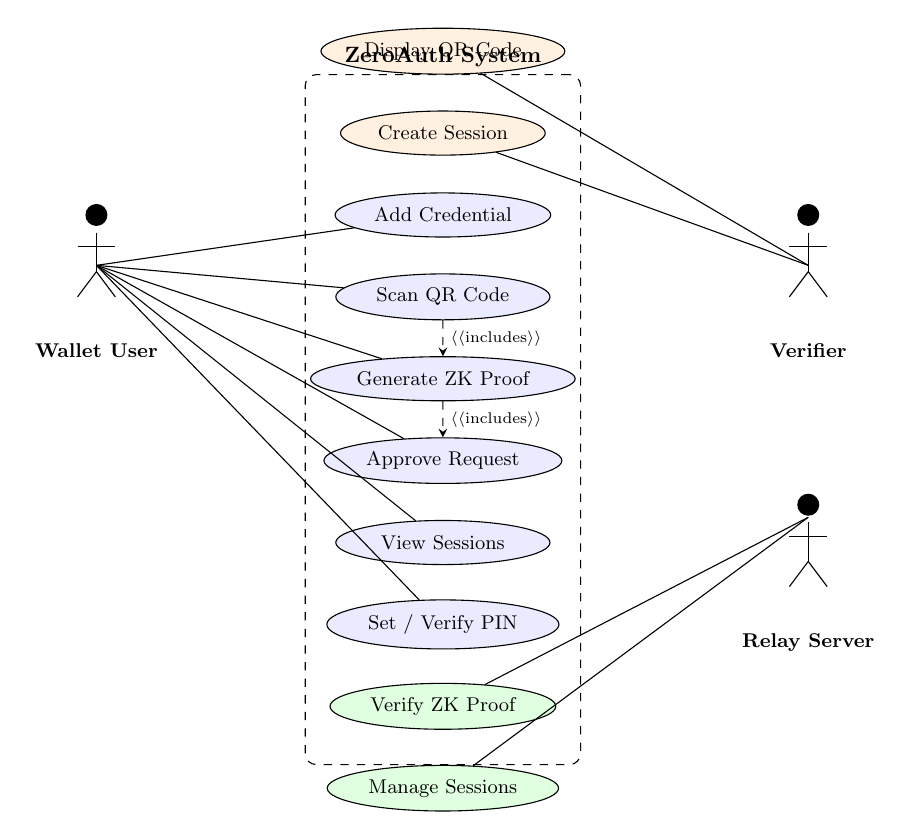
\begin{tikzpicture}[scale=0.80, every node/.style={scale=0.80}]

  % --- Actor: Wallet User ---
  \node[draw, circle, fill=black, minimum size=0.28cm] (uh) at (-5.5, 4.8) {};
  \draw (-5.5,4.52) -- (-5.5,3.9);
  \draw (-5.8,4.3) -- (-5.2,4.3);
  \draw (-5.5,3.9) -- (-5.8,3.5);
  \draw (-5.5,3.9) -- (-5.2,3.5);
  \node[font=\small, below=1.4cm of uh] {\textbf{Wallet User}};

  % --- Actor: Verifier ---
  \node[draw, circle, fill=black, minimum size=0.28cm] (vh) at (5.8, 4.8) {};
  \draw (5.8,4.52) -- (5.8,3.9);
  \draw (5.5,4.3) -- (6.1,4.3);
  \draw (5.8,3.9) -- (5.5,3.5);
  \draw (5.8,3.9) -- (6.1,3.5);
  \node[font=\small, below=1.4cm of vh] {\textbf{Verifier}};

  % --- Actor: Relay Server ---
  \node[draw, circle, fill=black, minimum size=0.28cm] (rh) at (5.8, 0.2) {};
  \draw (5.8,-0.08) -- (5.8,-0.7);
  \draw (5.5,-0.3) -- (6.1,-0.3);
  \draw (5.8,-0.7) -- (5.5,-1.1);
  \draw (5.8,-0.7) -- (6.1,-1.1);
  \node[font=\small, below=1.4cm of rh] {\textbf{Relay Server}};

  % Use cases
  \node[ellipse, draw, fill=blue!8, minimum width=3.4cm, minimum height=0.7cm,
        text centered, font=\small] (u1) at (0, 4.8) {Add Credential};
  \node[ellipse, draw, fill=blue!8, minimum width=3.4cm, minimum height=0.7cm,
        text centered, font=\small] (u2) at (0, 3.5) {Scan QR Code};
  \node[ellipse, draw, fill=blue!8, minimum width=3.4cm, minimum height=0.7cm,
        text centered, font=\small] (u3) at (0, 2.2) {Generate ZK Proof};
  \node[ellipse, draw, fill=blue!8, minimum width=3.4cm, minimum height=0.7cm,
        text centered, font=\small] (u4) at (0, 0.9) {Approve Request};
  \node[ellipse, draw, fill=blue!8, minimum width=3.4cm, minimum height=0.7cm,
        text centered, font=\small] (u5) at (0,-0.4) {View Sessions};
  \node[ellipse, draw, fill=blue!8, minimum width=3.4cm, minimum height=0.7cm,
        text centered, font=\small] (u6) at (0,-1.7) {Set / Verify PIN};

  \node[ellipse, draw, fill=orange!12, minimum width=3.2cm, minimum height=0.7cm,
        text centered, font=\small] (v1) at (0, 6.1) {Create Session};
  \node[ellipse, draw, fill=orange!12, minimum width=3.2cm, minimum height=0.7cm,
        text centered, font=\small] (v2) at (0, 7.4) {Display QR Code};

  \node[ellipse, draw, fill=green!12, minimum width=3.2cm, minimum height=0.7cm,
        text centered, font=\small] (r1) at (0,-3.0) {Verify ZK Proof};
  \node[ellipse, draw, fill=green!12, minimum width=3.2cm, minimum height=0.7cm,
        text centered, font=\small] (r2) at (0,-4.3) {Manage Sessions};

  % Connections
  \foreach \x in {u1,u2,u3,u4,u5,u6} \draw (-5.5,4.0) -- (\x);
  \foreach \x in {v1,v2}              \draw (5.8,4.0)  -- (\x);
  \foreach \x in {r1,r2}              \draw (5.8,0.0)  -- (\x);

  \draw[dashed,->,>=stealth] (u2) -- node[right,font=\scriptsize]{$\langle\langle$includes$\rangle\rangle$}(u3);
  \draw[dashed,->,>=stealth] (u3) -- node[right,font=\scriptsize]{$\langle\langle$includes$\rangle\rangle$}(u4);

  \node[draw, dashed, rounded corners,
        fit=(u1)(u2)(u3)(u4)(u5)(u6)(v1)(v2)(r1)(r2),
        inner sep=0.5cm, label=above:{\textbf{ZeroAuth System}}]{};
\end{tikzpicture}
\captionof{figure}{Use Case Diagram}
\label{fig:usecase}
\end{minipage}

\vspace{0.4cm}
Three actors interact with the ZeroAuth system. The Wallet User has six primary use cases: adding credentials to the local wallet, scanning verifier QR codes, generating ZK proofs, approving verification requests, viewing session history, and setting or verifying their device PIN. The Verifier actor, representing any third-party website using the SDK, creates verification sessions and displays QR codes. The Relay Server actor handles proof verification and manages the session lifecycle between PENDING and COMPLETED states. The $\langle\langle$includes$\rangle\rangle$ relationships between Scan QR Code, Generate ZK Proof, and Approve Request indicate that these steps are automatically chained together whenever the user initiates a scan.

% ═══════════════════════════════════════════════════════════════
\newpage
\section{Data Flow Diagram -- Level 0 (Context Diagram)}

\noindent\begin{minipage}{\linewidth}
\centering
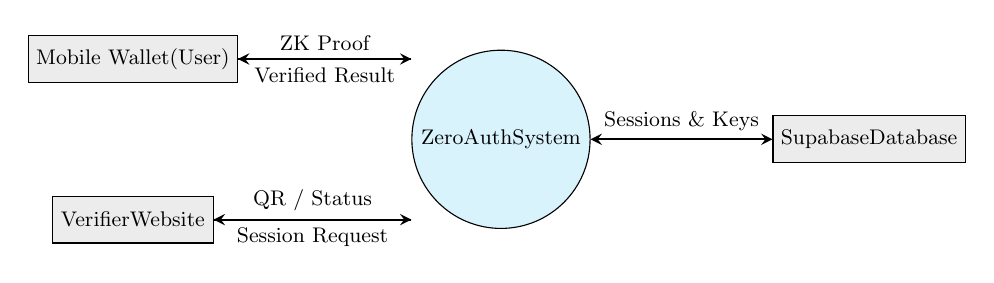
\begin{tikzpicture}[scale=0.85, every node/.style={scale=0.85},
    ext/.style={rectangle, draw, fill=gray!15, minimum width=2.4cm,
                minimum height=0.7cm, text centered, font=\small},
    proc/.style={circle, draw, fill=cyan!15, minimum size=2.6cm,
                 text centered, font=\small},
    arr/.style={->,>=stealth,thick}]

  \node[proc]  (sys)    at (0,0)    {ZeroAuth\\System};
  \node[ext]   (wallet) at (-5.5, 1.2) {Mobile Wallet\\(User)};
  \node[ext]   (web)    at (-5.5,-1.2) {Verifier\\Website};
  \node[ext]   (db)     at ( 5.5, 0)   {Supabase\\Database};

  \draw[arr] (wallet.east) -- node[above,font=\small]{ZK Proof} (sys.west |- wallet);
  \draw[arr] (sys.west |- wallet) -- node[below,font=\small]{Verified Result} (wallet.east);
  \draw[arr] (web.east) -- node[below,font=\small]{Session Request} (sys.west |- web);
  \draw[arr] (sys.west |- web) -- node[above,font=\small]{QR / Status} (web.east);
  \draw[arr,<->] (sys) -- node[above,font=\small]{Sessions \& Keys} (db);
\end{tikzpicture}
\captionof{figure}{DFD Level 0 -- Context Diagram}
\label{fig:dfd0}
\end{minipage}

\vspace{0.3cm}
The context diagram treats the entire ZeroAuth system as a single black-box process. The Mobile Wallet submits a Zero-Knowledge Proof and receives a verified result. The Verifier Website sends a session creation request and receives a QR payload and status updates. The Supabase Database provides bidirectional storage for sessions and verification keys.

\vspace{0.4cm}

% ─────────────────────────────────────────────────────────────
\subsection{DFD Level 1 -- Internal Processes}

\noindent\begin{minipage}{\linewidth}
\centering
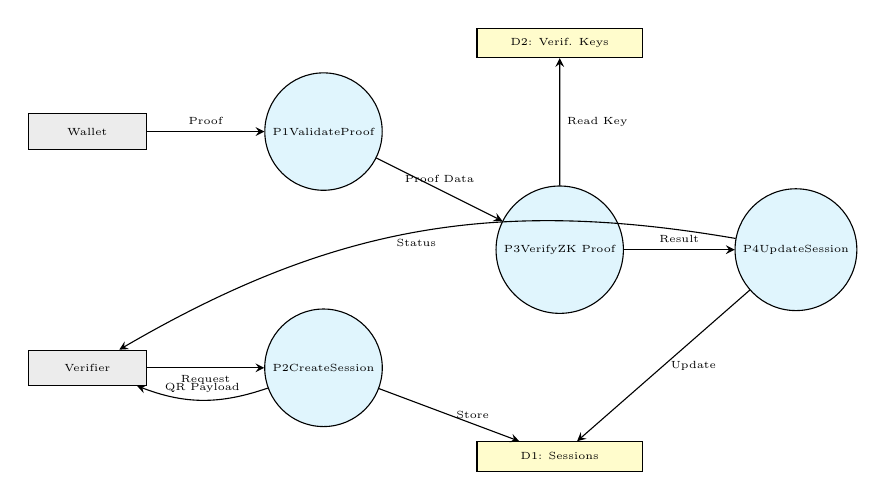
\begin{tikzpicture}[scale=0.75, every node/.style={scale=0.75},
    proc/.style={circle, draw, fill=cyan!12, minimum size=1.6cm,
                 text centered, font=\tiny},
    store/.style={rectangle, draw, fill=yellow!20, minimum width=2.8cm,
                  minimum height=0.5cm, text centered, font=\tiny},
    ext/.style={rectangle, draw, fill=gray!15, minimum width=2cm,
                minimum height=0.6cm, text centered, font=\tiny},
    arr/.style={->,>=stealth}]

  \node[ext]   (wallet) at (-6, 2)   {Wallet};
  \node[ext]   (web)    at (-6,-2)   {Verifier};
  \node[proc]  (p1)     at (-2, 2)   {P1\\Validate\\Proof};
  \node[proc]  (p2)     at (-2,-2)   {P2\\Create\\Session};
  \node[proc]  (p3)     at ( 2, 0)   {P3\\Verify\\ZK Proof};
  \node[proc]  (p4)     at ( 6, 0)   {P4\\Update\\Session};
  \node[store] (ds1)    at ( 2,-3.5) {D1: Sessions};
  \node[store] (ds2)    at ( 2, 3.5) {D2: Verif. Keys};

  \draw[arr] (wallet)--(p1) node[midway,above,font=\tiny]{Proof};
  \draw[arr] (web)--(p2)   node[midway,below,font=\tiny]{Request};
  \draw[arr] (p1)--(p3)   node[midway,above,font=\tiny]{Proof Data};
  \draw[arr] (p2)--(ds1)  node[midway,right,font=\tiny]{Store};
  \draw[arr] (p3)--(ds2)  node[midway,right,font=\tiny]{Read Key};
  \draw[arr] (p3)--(p4)   node[midway,above,font=\tiny]{Result};
  \draw[arr] (p4)--(ds1)  node[midway,right,font=\tiny]{Update};
  \draw[arr] (p4) to [bend right=20] node[below,font=\tiny]{Status} (web);
  \draw[arr] (p2) to [bend left=20]  node[above,font=\tiny]{QR Payload} (web);
\end{tikzpicture}
\captionof{figure}{DFD Level 1 -- Internal Processes}
\label{fig:dfd1}
\end{minipage}

\vspace{0.4cm}
The Level 1 DFD decomposes the system into four internal processes. Process P1 validates the structure and schema of incoming proof submissions from the Wallet, checking that all required fields are present and correctly formatted. Process P2 handles session creation requests from the Verifier, stores the new session record in data store D1, and returns a QR payload. Process P3 reads the appropriate Groth16 verification key from data store D2 and cryptographically verifies the submitted proof using snarkjs. Process P4 updates the session status in D1 to COMPLETED upon successful verification and sends the final result back to the Verifier.

% ═══════════════════════════════════════════════════════════════
\newpage
\section{Sequence Diagram}

\noindent\begin{minipage}{\linewidth}
\centering
\begin{tikzpicture}[scale=0.75, every node/.style={scale=0.75},
    life/.style={draw, fill=white, minimum width=1.5cm,
                 minimum height=0.5cm, text centered, font=\small\bfseries},
    msg/.style={->, >=stealth, font=\scriptsize}]

  \node[life, fill=orange!20] (W) at (0,  0) {Verifier};
  \node[life, fill=green!20]  (R) at (4,  0) {Relay};
  \node[life, fill=blue!15]   (M) at (8,  0) {Wallet};
  \node[life, fill=gray!15]   (D) at (12, 0) {Supabase};

  \foreach \x in {0,4,8,12}
    \draw[dashed, gray] (\x,-0.3) -- (\x,-11);

  \draw[msg] (0,-1.0) -- (4,-1.0)  node[midway,above]{① POST /sessions (credType)};
  \draw[msg] (4,-1.7) -- (12,-1.7) node[midway,above]{② INSERT session row};
  \draw[msg] (12,-2.4)-- (4,-2.4)  node[midway,above]{③ session\_id + nonce};
  \draw[msg] (4,-3.1) -- (0,-3.1)  node[midway,above]{④ QR payload (Base64)};
  \draw[msg] (0,-3.8) -- (8,-3.8)  node[midway,above]{⑤ Scan QR (camera)};
  \draw[->,>=stealth,font=\scriptsize,looseness=5]
        (8,-4.6) to [out=30,in=-30] node[right]{⑥ groth16.fullProve()} (8,-5.8);
  \draw[msg] (8,-6.5) -- (4,-6.5)  node[midway,above]{⑦ POST /sessions/:id/proof};
  \draw[msg] (4,-7.2) -- (12,-7.2) node[midway,above]{⑧ SELECT key\_data};
  \draw[msg] (12,-7.9)-- (4,-7.9)  node[midway,above]{⑨ verification key JSON};
  \node[font=\scriptsize,align=center] at (4.8,-8.6) {⑩ snarkjs.groth16.verify()};
  \draw[msg] (4,-9.3) -- (12,-9.3) node[midway,above]{⑪ UPDATE status=COMPLETED};
  \draw[msg] (4,-10.0)-- (8,-10.0) node[midway,above]{⑫ 200 OK};
  \draw[msg] (0,-10.6)-- (4,-10.6) node[midway,above]{⑬ GET /sessions/:id (poll)};
  \draw[msg] (4,-11.2)-- (0,-11.2) node[midway,above]{⑭ \{status: COMPLETED\}};
\end{tikzpicture}
\captionof{figure}{Sequence Diagram -- Verification Flow}
\label{fig:sequence}
\end{minipage}

\vspace{0.4cm}
The sequence diagram shows the full temporal interaction between the four system participants. The Verifier initiates the flow by posting a session creation request to the Relay (step 1), which stores the session in Supabase (step 2) and returns a session ID and nonce (step 3) encoded into a QR payload (step 4). The Wallet scans the QR code (step 5) and internally runs \texttt{groth16.fullProve()} to generate a cryptographic proof (step 6), which is then submitted to the Relay (step 7). The Relay retrieves the corresponding verification key from the database (steps 8--9), verifies the proof using snarkjs (step 10), and upon success updates the session status to COMPLETED in Supabase (step 11) before returning a 200 OK to the Wallet (step 12). The Verifier detects the completion through periodic polling (steps 13--14) and grants access to the authenticated user.

% ═══════════════════════════════════════════════════════════════
\newpage
\section{Flowchart -- Overall Verification Flow}

\noindent\begin{minipage}{\linewidth}
\centering
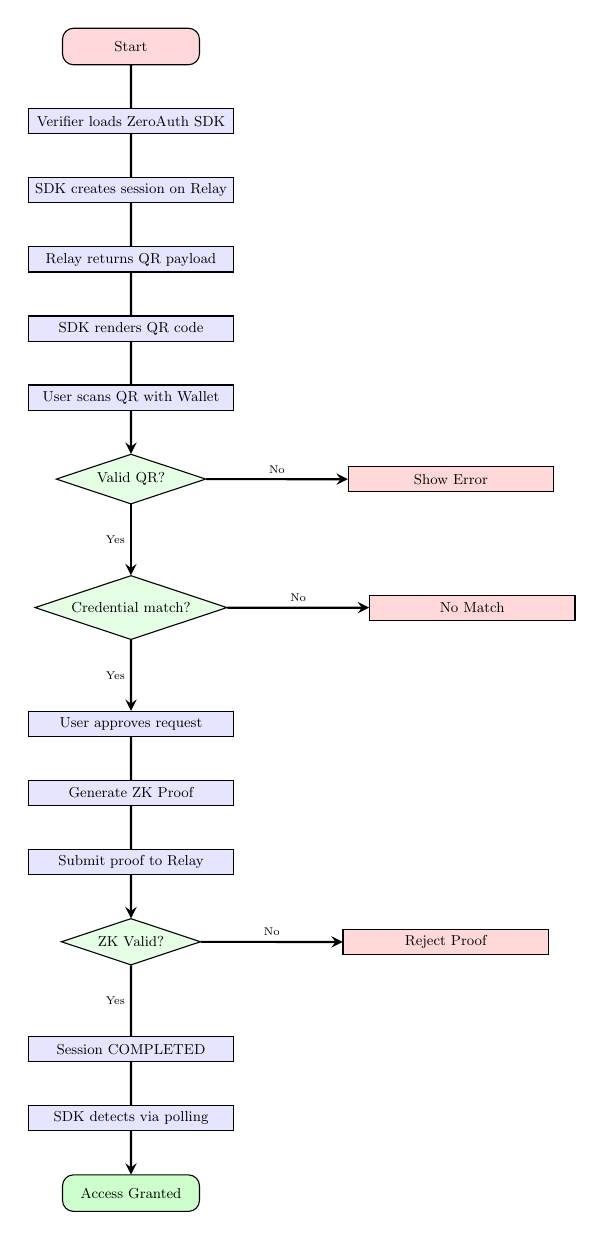
\begin{tikzpicture}[node distance=0.55cm, scale=0.58, every node/.style={scale=0.58},
    slim/.style={process, minimum width=4.5cm, minimum height=0.55cm, font=\small}]

  \node[startstop]  (s0) {Start};
  \node[slim, below=of s0]  (p1) {Verifier loads ZeroAuth SDK};
  \node[slim, below=of p1]  (p2) {SDK creates session on Relay};
  \node[slim, below=of p2]  (p3) {Relay returns QR payload};
  \node[slim, below=of p3]  (p4) {SDK renders QR code};
  \node[slim, below=of p4]  (p5) {User scans QR with Wallet};
  \node[decision, below=of p5, aspect=3, font=\small] (d1) {Valid QR?};
  \node[slim, right=1.8cm of d1, fill=red!15]  (e1) {Show Error};
  \node[decision, below=0.9cm of d1, aspect=3, font=\small] (d2) {Credential match?};
  \node[slim, right=1.8cm of d2, fill=red!15]  (e2) {No Match};
  \node[slim, below=0.9cm of d2]  (p6) {User approves request};
  \node[slim, below=of p6]  (p7) {Generate ZK Proof};
  \node[slim, below=of p7]  (p8) {Submit proof to Relay};
  \node[decision, below=of p8, aspect=3, font=\small] (d3) {ZK Valid?};
  \node[slim, right=1.8cm of d3, fill=red!15]  (e3) {Reject Proof};
  \node[slim, below=0.9cm of d3]  (p9) {Session COMPLETED};
  \node[slim, below=of p9]  (p10){SDK detects via polling};
  \node[startstop, below=of p10, fill=green!20] (s1) {Access Granted};

  \draw[arrow] (s0)--(p1)--(p2)--(p3)--(p4)--(p5)--(d1);
  \draw[arrow] (d1)--node[above,font=\scriptsize]{No} (e1);
  \draw[arrow] (d1)--node[left, font=\scriptsize]{Yes}(d2);
  \draw[arrow] (d2)--node[above,font=\scriptsize]{No} (e2);
  \draw[arrow] (d2)--node[left, font=\scriptsize]{Yes}(p6);
  \draw[arrow] (p6)--(p7)--(p8)--(d3);
  \draw[arrow] (d3)--node[above,font=\scriptsize]{No} (e3);
  \draw[arrow] (d3)--node[left, font=\scriptsize]{Yes}(p9)--(p10)--(s1);
\end{tikzpicture}
\captionof{figure}{Overall Verification Flowchart}
\label{fig:flowchart_main}
\end{minipage}

\vspace{0.3cm}
The overall verification flowchart captures the complete decision logic from session initiation to access grant. The Verifier website loads the SDK, which creates a session on the Relay and receives a QR payload that is rendered for the user. When the Wallet scans the QR code, the system first checks if the QR is valid and not expired. If valid, it checks whether the user has a credential that matches the requested type. On a successful credential match and user approval, the ZK proof is generated locally and submitted to the Relay. The Relay then performs cryptographic verification using snarkjs; an invalid proof is rejected immediately. On success, the session is marked COMPLETED, the SDK detects this via periodic polling, and the Verifier website grants access to the user. All failure paths terminate the flow early without any sensitive data disclosure.

% ═══════════════════════════════════════════════════════════════
\newpage
\section{ZK Proof Generation Flowchart}

\noindent\begin{minipage}{\linewidth}
\centering
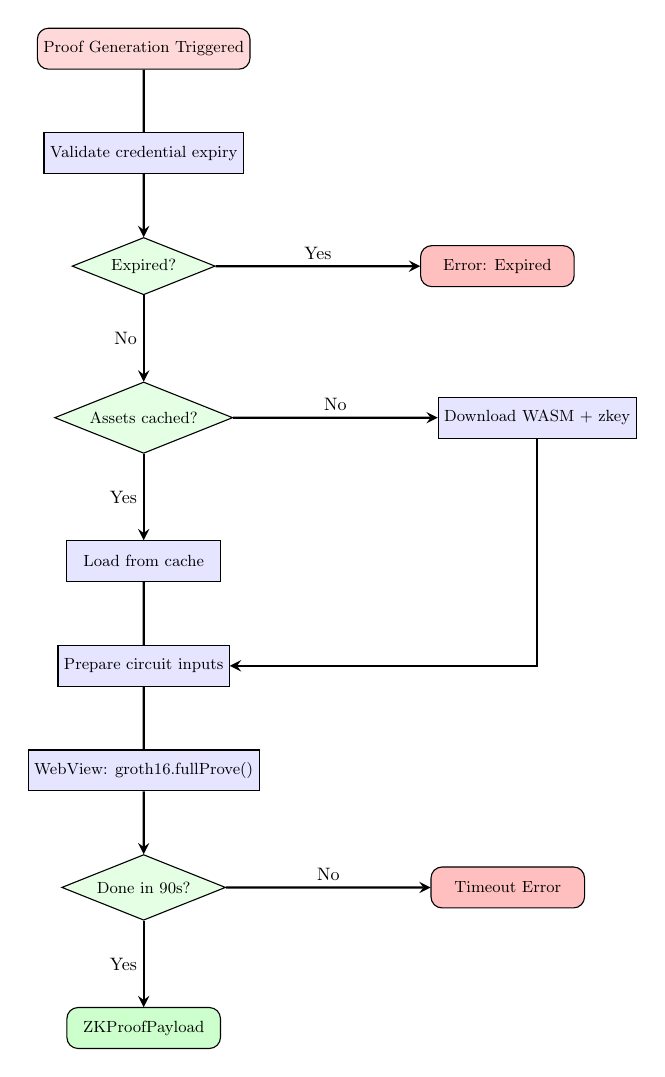
\begin{tikzpicture}[node distance=0.8cm, scale=0.65, every node/.style={scale=0.65}]
  \node[startstop] (s0) {Proof Generation Triggered};
  \node[process, below=of s0]   (p1) {Validate credential expiry};
  \node[decision, below=of p1, aspect=2.5]  (d1) {Expired?};
  \node[startstop, right=2.6cm of d1, fill=red!25] (e1) {Error: Expired};
  \node[decision, below=1.1cm of d1, aspect=2.5]  (d2) {Assets cached?};
  \node[process, right=2.6cm of d2] (p2) {Download WASM + zkey};
  \node[process, below=1.1cm of d2] (p3) {Load from cache};
  \node[process, below=of p3]  (p4) {Prepare circuit inputs};
  \node[process, below=of p4]  (p5) {WebView: groth16.fullProve()};
  \node[decision, below=of p5, aspect=2.5]  (d3) {Done in 90s?};
  \node[startstop, right=2.6cm of d3, fill=red!25] (e2) {Timeout Error};
  \node[startstop, below=1.1cm of d3, fill=green!20] (s1) {ZKProofPayload};

  \draw[arrow] (s0)--(p1)--(d1);
  \draw[arrow] (d1)--node[above]{Yes}(e1);
  \draw[arrow] (d1)--node[left]{No}(d2);
  \draw[arrow] (d2)--node[above]{No}(p2);
  \draw[arrow] (d2)--node[left]{Yes}(p3);
  \draw[arrow] (p2)|-(p4);
  \draw[arrow] (p3)--(p4)--(p5)--(d3);
  \draw[arrow] (d3)--node[above]{No}(e2);
  \draw[arrow] (d3)--node[left]{Yes}(s1);
\end{tikzpicture}
\captionof{figure}{ZK Proof Generation Flowchart}
\label{fig:flowchart_zk}
\end{minipage}

\vspace{0.4cm}
This flowchart details the internal proof generation process within the mobile Wallet. The process begins by validating whether the selected credential has expired, immediately terminating with an error if it has. Next, the system checks whether the WASM circuit file and zkey file are cached locally from a previous run. If not cached, they are downloaded from the bundled assets and stored for future use. The circuit inputs, which include values such as the birth year, random salt, current year, and minimum age threshold, are then prepared and passed to a sandboxed WebView bridge which executes \texttt{snarkjs.groth16.fullProve()}. A 90-second timeout is enforced to accommodate low-end devices. On successful completion within the time limit, a ZKProofPayload containing the proof elements $\pi_a$, $\pi_b$, $\pi_c$ and the public signals is returned for submission to the Relay.

% ═══════════════════════════════════════════════════════════════
\newpage
\section{Block Diagram}

\noindent\begin{minipage}{\linewidth}
\centering
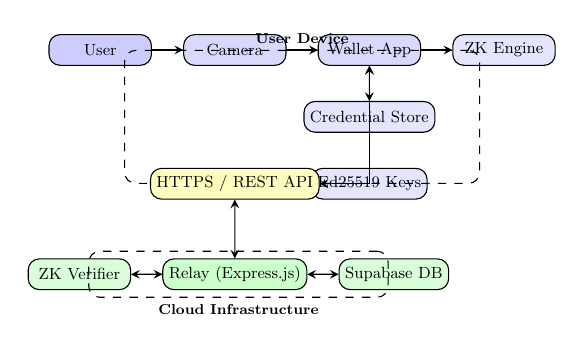
\begin{tikzpicture}[node distance=0.5cm, scale=0.65, every node/.style={scale=0.65},
    blk/.style={draw, rounded corners, fill=#1, minimum width=2.0cm,
                minimum height=0.6cm, text centered, font=\small}]

  \node[blk=blue!20] (usr)  {User};
  \node[blk=blue!15, right=0.4cm of usr]  (cam)  {Camera};
  \node[blk=blue!15, right=0.4cm of cam]  (wapp) {Wallet App};
  \node[blk=blue!10, below=0.45cm of wapp] (crd) {Credential Store};
  \node[blk=blue!10, right=0.4cm of wapp] (zke)  {ZK Engine};
  \node[blk=blue!10, below=0.45cm of crd] (key)  {Ed25519 Keys};
  \node[draw,dashed,rounded corners,
        fit=(usr)(cam)(wapp)(crd)(zke)(key), inner sep=0.25cm,
        label=above:{\footnotesize\textbf{User Device}}]{};

  \node[blk=yellow!25, below=1.3cm of cam, minimum width=3.2cm] (net) {HTTPS / REST API};

  \node[blk=green!20, below=0.75cm of net] (rel) {Relay (Express.js)};
  \node[blk=green!15, left=0.4cm  of rel]  (zkv) {ZK Verifier};
  \node[blk=green!15, right=0.4cm of rel]  (sup) {Supabase DB};
  \node[draw,dashed,rounded corners,
        fit=(rel)(zkv)(sup), inner sep=0.25cm,
        label=below:{\footnotesize\textbf{Cloud Infrastructure}}]{};

  \draw[->,>=stealth] (usr)--(cam);
  \draw[->,>=stealth] (cam)--(wapp);
  \draw[<->,>=stealth] (wapp)--(crd);
  \draw[->,>=stealth] (wapp)--(zke);
  \draw[<->,>=stealth] (wapp)|-(net);
  \draw[<->,>=stealth] (net)--(rel);
  \draw[<->,>=stealth] (rel)--(zkv);
  \draw[<->,>=stealth] (rel)--(sup);
\end{tikzpicture}
\captionof{figure}{Block Diagram}
\label{fig:block}
\end{minipage}

\vspace{0.3cm}
The block diagram illustrates the physical and logical separation of the ZeroAuth system across two tiers. The User Device layer contains the Wallet application, which interfaces with the camera for QR scanning, the Credential Store for local data persistence, the ZK Engine for proof generation, and the Ed25519 key module for identity management. All proof-related communication between the device and the cloud is channelled exclusively through the HTTPS REST API layer, ensuring that no raw credential data crosses this boundary. The Cloud Infrastructure layer contains the Express.js Relay server, the snarkjs ZK Verifier component for cryptographic proof validation, and the Supabase PostgreSQL database for session and verification key storage.

\vspace{0.5cm}

% ─────────────────────────────────────────────────────────────
\section{Database Schema (ER Diagram)}

\noindent\begin{minipage}{\linewidth}
\centering
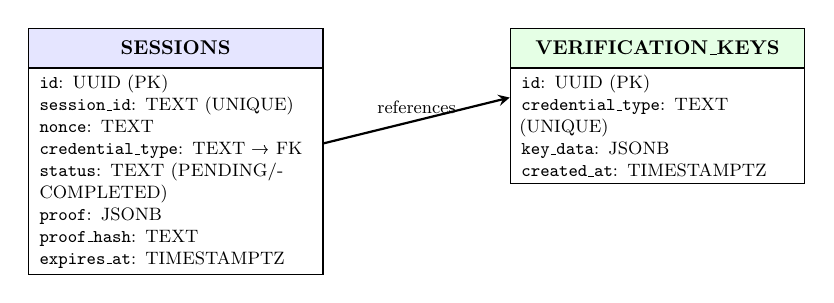
\begin{tikzpicture}[scale=0.72, every node/.style={scale=0.72}]
  \node[draw, fill=blue!10, minimum width=5.2cm, minimum height=0.7cm,
        text centered, font=\normalsize\bfseries] (st) at (0,0) {SESSIONS};
  \node[draw, below=0cm of st, minimum width=5.2cm, text width=4.8cm,
        font=\small, align=left] (sf) {
    \texttt{id}: UUID (PK)\\
    \texttt{session\_id}: TEXT (UNIQUE)\\
    \texttt{nonce}: TEXT\\
    \texttt{credential\_type}: TEXT \textrightarrow\ FK\\
    \texttt{status}: TEXT (PENDING/COMPLETED)\\
    \texttt{proof}: JSONB\\
    \texttt{proof\_hash}: TEXT\\
    \texttt{expires\_at}: TIMESTAMPTZ
  };

  \node[draw, fill=green!10, minimum width=5.2cm, minimum height=0.7cm,
        text centered, font=\normalsize\bfseries] (vt) at (8.5,0) {VERIFICATION\_KEYS};
  \node[draw, below=0cm of vt, minimum width=5.2cm, text width=4.8cm,
        font=\small, align=left] (vf) {
    \texttt{id}: UUID (PK)\\
    \texttt{credential\_type}: TEXT (UNIQUE)\\
    \texttt{key\_data}: JSONB\\
    \texttt{created\_at}: TIMESTAMPTZ
  };

  \draw[->,>=stealth,thick]
    ([yshift=0.5cm]sf.east) --
    node[above,font=\small]{references}
    ([yshift=0.5cm]vf.west);
\end{tikzpicture}
\captionof{figure}{Database ER Diagram}
\label{fig:er}
\end{minipage}

\vspace{0.3cm}
The database schema consists of two tables managed within Supabase PostgreSQL, both protected by Row-Level Security policies that restrict access exclusively to the Relay service role. The SESSIONS table records every verification request, storing the unique session identifier, a cryptographic nonce to prevent replay attacks, the credential type requested, the current session status (PENDING or COMPLETED), the submitted ZK proof in JSONB format, a SHA-256 hash of the proof for deduplication, and the session expiry timestamp. The VERIFICATION\_KEYS table holds the Groth16 verification key for each supported credential type as a JSONB object. The \texttt{credential\_type} field in SESSIONS acts as a foreign key reference to VERIFICATION\_KEYS, enabling the Relay to dynamically load the correct verification key at proof submission time without hardcoding per-circuit logic.
\end{minipage}

\chapter{System Implementation}

The project is implemented as a three-component privacy-preserving authentication system. The implementation involves cryptographic circuit design, mobile app development, server-side proof verification, and web SDK integration. This chapter describes each component's implementation in detail with code listings and architectural insights.

\section{Development Environment Setup}

Before beginning the core implementation, a consistent development environment was established across all components:

\begin{lstlisting}[language=bash, caption={Development Environment Initialization}]
# Install Node.js 18 LTS
nvm install 18
nvm use 18

# Install Expo CLI for mobile development
npm install -g expo-cli eas-cli

# Install Circom compiler
cargo install circom

# Install snarkjs globally
npm install -g snarkjs

# Verify installations
node --version   # v18.x.x
circom --version # circom compiler 2.0.x
snarkjs --version  # 0.7.x
\end{lstlisting}

\section{Wallet Application}

The Wallet is a React Native/Expo mobile application that serves as the user's identity container and proof generator. Its file structure is organized as follows:

\begin{lstlisting}[language=bash, caption={Wallet Application File Structure}]
wallet/
  app/
    (tabs)/
      index.tsx       # Credentials home screen
      sessions.tsx    # Session history screen
      settings.tsx    # Settings screen
  components/
    CredentialCard.tsx
    ProofModal.tsx
    QRScanner.tsx
  hooks/
    useCredentialStore.ts
    useNetworkStatus.ts
    useProofEngine.ts
  lib/
    wallet.ts         # Ed25519 identity
    zkbridge.ts       # WebView ZK proof bridge
    crypto.ts         # Hashing utilities
    revocation.ts     # Revocation checking
  circuits/
    age_check.wasm
    age_check.zkey
    student_check.wasm
    student_check.zkey
  assets/
    zkwebview.html    # Sandboxed ZK environment
\end{lstlisting}

\subsection{Identity Management (Ed25519)}

The wallet generates an Ed25519 keypair on first launch for decentralized identity:

\begin{lstlisting}[language=Java, caption={Identity Generation (wallet.ts)}]
export async function generateAndStoreIdentity() {
    const privateKey = new Uint8Array(32);
    getRandomValues(privateKey);
    const publicKey = ed25519.getPublicKey(privateKey);
    
    // Store securely in platform SecureStore
    await SecureStore.setItemAsync(
        PRIVATE_KEY_ALIAS, toBase64(privateKey)
    );
    
    // Derive W3C did:key identifier
    const did = deriveDID(publicKey); // "did:key:z..."
    return { publicKey, did };
}

function deriveDID(publicKey: Uint8Array): string {
    // Prepend multicodec prefix 0xed01
    const multicodec = new Uint8Array([0xed, 0x01, ...publicKey]);
    // Encode with Base58BTC
    const b58 = base58btc.encode(multicodec);
    return `did:key:z${b58}`;
}
\end{lstlisting}

The DID is derived following the \textbf{W3C did:key specification}: the Ed25519 public key is prepended with the multicodec prefix \texttt{0xed01}, encoded in Base58BTC, and prefixed with \texttt{did:key:z}.

\subsection{Credential Storage}

Credentials are stored locally using Zustand state management with AsyncStorage persistence. Table 5.1 below describes each field in the credential data structure stored within the wallet.

\begin{table}[H]
\centering
\caption{Credential Structure}
\begin{tabular}{|l|p{8cm}|}
\hline
\textbf{Field} & \textbf{Description} \\
\hline
\texttt{id} & Unique identifier (cryptographically generated) \\
\texttt{type} & Credential type (Age Verification, Student ID, Trial) \\
\texttt{issuer} & Name of the issuing authority \\
\texttt{attributes} & Key-value pairs (e.g., birth\_year: ``1995'') \\
\texttt{commitments} & Poseidon hash commitments binding attributes \\
\texttt{expiresAt} & Optional expiration timestamp \\
\texttt{revocationId} & Optional ID for revocation checking \\
\hline
\end{tabular}
\end{table}

\begin{lstlisting}[language=Java, caption={Credential Store (useCredentialStore.ts)}]
interface Credential {
  id: string;
  type: 'Age Verification' | 'Student ID' | 'Trial';
  issuer: string;
  attributes: Record<string, string | number | boolean>;
  commitments: Record<string, bigint>;
  expiresAt?: number;
  revocationId?: string;
}

const useCredentialStore = create<CredentialStore>()(
  persist(
    (set, get) => ({
      credentials: [],
      addCredential: (cred: Credential) =>
        set(s => ({ credentials: [...s.credentials, cred] })),
      removeCredential: (id: string) =>
        set(s => ({
          credentials: s.credentials.filter(c => c.id !== id)
        })),
    }),
    { name: 'credentials', storage: createJSONStorage(() => AsyncStorage) }
  )
);
\end{lstlisting}

\subsection{PIN-based Protection}

The wallet is protected by a PIN with security-hardened storage using SHA-256 hashing with unique salts. PIN verification uses \textbf{timing-safe comparison} to prevent timing side-channel attacks:

\begin{lstlisting}[language=Java, caption={Timing-safe PIN verification (utils.ts)}]
export async function verifyPin(
    pin: string, storedValue: string
): Promise<boolean> {
    const [salt, storedHash] = storedValue.split(':');
    const inputHash = await digestStringAsync(
        CryptoDigestAlgorithm.SHA256, pin + salt
    );
    // Timing-safe comparison
    let result = 0;
    for (let i = 0; i < inputHash.length; i++) {
        result |= inputHash.charCodeAt(i) 
                 ^ storedHash.charCodeAt(i);
    }
    return result === 0;
}

export async function hashPin(pin: string): Promise<string> {
    // Generate random 16-byte salt
    const salt = toHex(getRandomValues(new Uint8Array(16)));
    const hash = await digestStringAsync(
        CryptoDigestAlgorithm.SHA256, pin + salt
    );
    return `${salt}:${hash}`;
}
\end{lstlisting}

\subsection{QR Scanner and Session Parsing}

When a user opens the Wallet and taps ``Scan QR Code'', the camera module activates and scans the QR code displayed on the verifier website:

\begin{lstlisting}[language=Java, caption={QR Code Parsing (QRScanner.tsx)}]
function parseQRPayload(rawData: string): QRPayload {
  const decoded = atob(rawData);
  const payload: QRPayload = JSON.parse(decoded);
  
  // Validate protocol version
  if (payload.v !== 1) throw new Error('Unsupported protocol version');
  
  // Check expiration
  const now = Math.floor(Date.now() / 1000);
  if (payload.expires_at < now) throw new Error('QR code expired');
  
  // Validate required fields
  if (!payload.session_id || !payload.nonce || 
      !payload.credential_type) {
    throw new Error('Invalid QR payload structure');
  }
  return payload;
}
\end{lstlisting}

\section{ZK Circuit Design}

\subsection{Age Verification Circuit}

The \texttt{age\_check.circom} circuit implements age verification with Poseidon commitment binding:

\begin{lstlisting}[language=C, caption={Age Verification Circuit (age\_check.circom)}]
pragma circom 2.0.0;

include "node_modules/circomlib/circuits/poseidon.circom";
include "node_modules/circomlib/circuits/comparators.circom";

template AgeCheck() {
    signal input currentYear;    // Public
    signal input minAge;         // Public
    signal input birthYear;      // Private
    signal input salt;           // Private
    signal input commitment;     // Public

    // 1. Verify Commitment: commitment = Poseidon(birthYear, salt)
    component hasher = Poseidon(2);
    hasher.inputs[0] <== birthYear;
    hasher.inputs[1] <== salt;
    hasher.out === commitment;

    // 2. Age Check: currentYear - birthYear >= minAge
    signal age;
    age <== currentYear - birthYear;
    component ge = GreaterEqThan(32);
    ge.in[0] <== age;
    ge.in[1] <== minAge;
    ge.out === 1;
}

component main {public [currentYear, minAge, commitment]} = AgeCheck();
\end{lstlisting}

\subsection{Student ID Verification Circuit}

The \texttt{student\_check.circom} circuit verifies active student status using a 3-input Poseidon hash commitment:

\begin{lstlisting}[language=C, caption={Student ID Circuit (student\_check.circom)}]
pragma circom 2.0.0;

include "node_modules/circomlib/circuits/poseidon.circom";
include "node_modules/circomlib/circuits/comparators.circom";

template StudentCheck() {
    signal input currentYear;    // Public
    signal input commitment;     // Public
    signal input isStudent;      // Private (must be 1)
    signal input expiryYear;     // Private
    signal input salt;           // Private

    // 1. Verify commitment
    component hasher = Poseidon(3);
    hasher.inputs[0] <== isStudent;
    hasher.inputs[1] <== expiryYear;
    hasher.inputs[2] <== salt;
    hasher.out === commitment;

    // 2. isStudent === 1
    isStudent === 1;

    // 3. expiryYear >= currentYear (not expired)
    component ge = GreaterEqThan(32);
    ge.in[0] <== expiryYear;
    ge.in[1] <== currentYear;
    ge.out === 1;
}

component main {public [currentYear, commitment]} = StudentCheck();
\end{lstlisting}

\subsection{Circuit Compilation and Trusted Setup}

\begin{lstlisting}[language=bash, caption={Circuit Compilation Steps}]
# Compile circuit to R1CS and WASM
circom age_check.circom --r1cs --wasm --sym

# Download Powers of Tau (Phase 1 trusted setup)
wget https://hermez.s3-eu-west-1.amazonaws.com/powersOfTau28_hez_final_14.ptau

# Phase 2 setup for circuit
snarkjs groth16 setup age_check.r1cs \
    powersOfTau28_hez_final_14.ptau \
    age_check_0.zkey

# Contribute to trusted setup (add randomness)
snarkjs zkey contribute age_check_0.zkey \
    age_check_final.zkey --name="ZeroAuth Setup"

# Export verification key
snarkjs zkey export verificationkey \
    age_check_final.zkey verification_key.json

# Export Solidity verifier (for future on-chain use)
snarkjs zkey export solidityverifier \
    age_check_final.zkey AgeVerifier.sol
\end{lstlisting}

\subsection{WebView ZK Proof Bridge}

Since snarkjs runs in a browser environment (WebView), a JavaScript bridge connects the React Native app to the proof generation engine:

\begin{lstlisting}[language=Java, caption={ZK WebView Bridge (zkbridge.ts)}]
export async function generateProof(
    credType: string,
    inputs: ProofInputs,
    timeout = 90000
): Promise<ZKProofPayload> {
    return new Promise((resolve, reject) => {
        const timer = setTimeout(
            () => reject(new Error('Proof timeout')), timeout
        );
        
        webViewRef.current?.injectJavaScript(`
            (async () => {
                try {
                    const { proof, publicSignals } = 
                        await snarkjs.groth16.fullProve(
                            ${JSON.stringify(inputs)},
                            '${credType}_check.wasm',
                            '${credType}_check.zkey'
                        );
                    window.ReactNativeWebView.postMessage(
                        JSON.stringify({ success: true, 
                            proof, publicSignals })
                    );
                } catch (e) {
                    window.ReactNativeWebView.postMessage(
                        JSON.stringify({ success: false, 
                            error: e.message })
                    );
                }
            })();
        `);
        
        // onMessage handler resolves/rejects the promise
        setOnMessage((data) => {
            clearTimeout(timer);
            if (data.success) resolve(data);
            else reject(new Error(data.error));
        });
    });
}
\end{lstlisting}

\section{Relay Server}

The Relay is a Node.js/Express server that manages verification sessions and verifies ZK proofs.

\subsection{Server Architecture}

\begin{lstlisting}[language=bash, caption={Relay Server File Structure}]
relay/
  src/
    index.ts           # Express app entry point
    routes/
      sessions.ts      # Session CRUD + proof submission
    middleware/
      rateLimiter.ts   # express-rate-limit config
      errorHandler.ts  # Global error middleware
      logger.ts        # Request logging
    services/
      supabase.ts      # Database client
      zkVerifier.ts    # snarkjs proof verification
      sessionService.ts # Session lifecycle management
    utils/
      proofHash.ts     # SHA-256 proof hashing
      cleanup.ts       # Expired session cleanup job
\end{lstlisting}

\subsection{Session Management}

Sessions follow a lifecycle: \texttt{PENDING} $\rightarrow$ \texttt{COMPLETED} $\rightarrow$ \texttt{expired/deleted}. New sessions are created with a 5-minute TTL. Expired sessions are automatically cleaned up every 60 seconds.

\begin{lstlisting}[language=Java, caption={Session Creation (sessionService.ts)}]
export async function createSession(
    credentialType: string,
    verifierName: string,
    requiredClaims: string[],
    expirySeconds = 300
): Promise<Session> {
    const sessionId = uuidv4();
    const nonce = crypto.randomBytes(32).toString('hex');
    const expiresAt = new Date(
        Date.now() + expirySeconds * 1000
    ).toISOString();
    
    const { data, error } = await supabase
        .from('sessions')
        .insert({
            session_id: sessionId,
            nonce,
            verifier_name: verifierName,
            required_claims: requiredClaims,
            credential_type: credentialType,
            status: 'PENDING',
            expires_at: expiresAt
        })
        .select()
        .single();
    
    if (error) throw new Error(`DB insert failed: ${error.message}`);
    return data;
}
\end{lstlisting}

\subsection{Proof Verification Pipeline}

When a proof is submitted, it passes through a multi-stage verification pipeline:

\begin{enumerate}
    \item \textbf{Session Validation}: Check session exists and is PENDING.
    \item \textbf{Schema Validation}: Verify proof structure ($\pi_a$, $\pi_b$, $\pi_c$ arrays).
    \item \textbf{Replay Protection}: Compute SHA-256 hash and check for duplicates.
    \item \textbf{ZK Verification}: Cryptographically verify using \texttt{snarkjs.groth16.verify()}.
    \item \textbf{Session Update}: Mark session as COMPLETED with proof data.
\end{enumerate}

\begin{lstlisting}[language=Java, caption={Proof Verification (zkVerifier.ts)}]
export async function verifyProof(
    sessionId: string,
    proof: ZKProof,
    publicSignals: string[]
): Promise<boolean> {
    // 1. Load verification key from database
    const { data: keyData } = await supabase
        .from('verification_keys')
        .select('key_data')
        .eq('credential_type', session.credential_type)
        .single();
    
    // 2. Compute proof hash for replay check
    const proofHash = computeProofHash(proof, publicSignals);
    if (await isProofUsed(proofHash)) {
        throw new Error('Proof replay detected');
    }
    
    // 3. Verify with snarkjs
    const isValid = await snarkjs.groth16.verify(
        keyData.key_data,
        publicSignals,
        proof
    );
    
    if (!isValid) throw new Error('Invalid ZK proof');
    
    // 4. Mark session completed
    await supabase.from('sessions')
        .update({ 
            status: 'COMPLETED', 
            proof, proof_hash: proofHash 
        })
        .eq('session_id', sessionId);
    
    return true;
}

function computeProofHash(
    proof: ZKProof, 
    publicSignals: string[]
): string {
    const canonical = JSON.stringify({
        pi_a: proof.pi_a.sort(),
        pi_b: proof.pi_b.map(p => p.sort()).sort(),
        pi_c: proof.pi_c.sort(),
        publicSignals: publicSignals.sort()
    });
    return crypto.createHash('sha256')
        .update(canonical).digest('hex');
}
\end{lstlisting}

\subsection{Security Measures}

The Relay server incorporates multiple independent security mechanisms to protect against common attack vectors. Table 5.2 below summarises each measure and its corresponding implementation.

\begin{table}[H]
\centering
\caption{Relay Server Security Measures}
\begin{tabular}{|l|p{7cm}|}
\hline
\textbf{Security Measure} & \textbf{Implementation} \\
\hline
Rate Limiting & 500 requests per IP per 15 minutes \\
Request Size Limit & 10MB max body, 1MB max proof payload \\
Session Expiry & 5-minute TTL with automatic cleanup \\
Proof Replay Protection & SHA-256 hash deduplication \\
Row-Level Security & Supabase RLS policies on all tables \\
CORS & Enabled for cross-origin SDK access \\
Request Logging & Timestamp, method, path, IP logged \\
Error Sanitization & Internal errors never exposed to client \\
HTTPS Only & HTTP redirected to HTTPS in production \\
\hline
\end{tabular}
\end{table}

\section{Web SDK}

The SDK provides two integration methods for verifier websites:

\subsection{React Component Integration}
\begin{lstlisting}[language=HTML, caption={React Integration}]
import { ZeroAuthButton } from '@zero-auth/sdk';

// Basic usage
<ZeroAuthButton 
  credentialType="Age Verification"
  claims={['birth_year']}
  onSuccess={(result) => {
    console.log('Verified!', result);
    // Grant access to user
    setVerified(true);
  }}
  onError={(err) => {
    console.error('Verification failed:', err);
  }}
/>

// With custom relay URL
<ZeroAuthButton 
  relayUrl="https://your-relay.example.com"
  credentialType="Student ID"
  claims={['isStudent', 'expiryYear']}
  onSuccess={handleSuccess}
  verifierName="University Bookstore"
/>
\end{lstlisting}

\subsection{CDN / Vanilla JavaScript Integration}
\begin{lstlisting}[language=HTML, caption={CDN Integration}]
<script src="https://unpkg.com/@zero-auth/sdk/dist/
  zero-auth-sdk.umd.js"></script>
<script>
  window.ZeroAuthConfig = {
    relayUrl: 'https://zeroauth-relay.onrender.com',
    verifierName: 'My Website'
  };
  
  ZeroAuth.createButton({
    elementId: 'verify-btn',
    credentialType: 'Age Verification',
    claims: ['birth_year'],
    onSuccess: function(result) {
      document.getElementById('content').style.display = 'block';
    }
  });
</script>

<div id="verify-btn"></div>
<div id="content" style="display:none">
  <!-- Age-restricted content -->
</div>
\end{lstlisting}

\subsection{SDK Session Polling Implementation}

\begin{lstlisting}[language=Java, caption={Session Polling (sdk/polling.ts)}]
export async function pollSessionStatus(
    sessionId: string,
    relayUrl: string,
    intervalMs = 2000,
    timeoutMs = 300000
): Promise<SessionResult> {
    const startTime = Date.now();
    
    while (Date.now() - startTime < timeoutMs) {
        const res = await fetch(
            `${relayUrl}/api/v1/sessions/${sessionId}`
        );
        const data = await res.json();
        
        if (data.status === 'COMPLETED') {
            return { success: true, ...data };
        }
        if (data.status === 'EXPIRED' || data.status === 'REJECTED') {
            throw new Error(`Session ${data.status}`);
        }
        
        // Wait before next poll
        await new Promise(r => setTimeout(r, intervalMs));
    }
    throw new Error('Verification timeout');
}
\end{lstlisting}

\section{QR Code Protocol}

The verification protocol uses a structured JSON payload encoded in QR codes:

\begin{lstlisting}[language=Java, caption={QR Code Payload Structure}]
{
  "v": 1,
  "action": "verify",
  "session_id": "550e8400-e29b-41d4-a716-446655440000",
  "nonce": "a3f2...<64 hex chars>",
  "verifier": {
    "name": "Example Age-Gated Service",
    "did": "did:web:example.com",
    "callback": "https://relay/api/v1/sessions/{id}/proof"
  },
  "required_claims": ["birth_year"],
  "credential_type": "Age Verification",
  "expires_at": 1712345678
}
\end{lstlisting}

\section{Security Implementation Details}

\subsection{Proof Replay Protection}

Each proof is hashed using SHA-256 with deterministic key ordering. If a proof hash matches a previously submitted proof for the same session, the submission is rejected.

\subsection{Credential Revocation}

The wallet supports offline-capable revocation checking with a 1-hour cache duration. Revocation status is checked before generating proofs and cached in AsyncStorage for offline scenarios.

\subsection{Offline Queue}

When network connectivity is unavailable, actions are queued and automatically processed upon reconnection using the \texttt{useNetworkStatus} hook that monitors connectivity changes via \texttt{NetInfo}.

\begin{lstlisting}[language=Java, caption={Offline Queue (useNetworkStatus.ts)}]
export function useNetworkStatus() {
  const [isOnline, setIsOnline] = useState(true);
  const queueRef = useRef<QueuedAction[]>([]);

  useEffect(() => {
    const unsub = NetInfo.addEventListener(state => {
      const online = state.isConnected && state.isInternetReachable;
      if (online && !isOnline) {
        // Process queued actions on reconnect
        processQueue(queueRef.current).then(() => {
          queueRef.current = [];
        });
      }
      setIsOnline(online ?? false);
    });
    return unsub;
  }, [isOnline]);

  const enqueue = (action: QueuedAction) => {
    queueRef.current.push(action);
  };

  return { isOnline, enqueue };
}
\end{lstlisting}

\section{Database Implementation}

The Supabase PostgreSQL schema is set up with the following SQL statements:

\begin{lstlisting}[language=SQL, caption={Database Schema DDL}]
-- Sessions table
CREATE TABLE sessions (
    id UUID PRIMARY KEY DEFAULT gen_random_uuid(),
    session_id TEXT UNIQUE NOT NULL,
    nonce TEXT NOT NULL,
    verifier_name TEXT,
    required_claims JSONB NOT NULL DEFAULT '[]',
    credential_type TEXT NOT NULL,
    status TEXT NOT NULL DEFAULT 'PENDING'
        CHECK (status IN ('PENDING','COMPLETED','EXPIRED')),
    proof JSONB,
    proof_hash TEXT,
    created_at TIMESTAMPTZ NOT NULL DEFAULT NOW(),
    expires_at TIMESTAMPTZ NOT NULL
);

-- Auto-expire index
CREATE INDEX idx_sessions_expires ON sessions(expires_at);
CREATE INDEX idx_sessions_status ON sessions(status);

-- Verification keys table  
CREATE TABLE verification_keys (
    id UUID PRIMARY KEY DEFAULT gen_random_uuid(),
    credential_type TEXT UNIQUE NOT NULL,
    key_data JSONB NOT NULL,
    created_at TIMESTAMPTZ NOT NULL DEFAULT NOW()
);

-- Row Level Security
ALTER TABLE sessions ENABLE ROW LEVEL SECURITY;
ALTER TABLE verification_keys ENABLE ROW LEVEL SECURITY;

-- Allow relay service role full access
CREATE POLICY "service_role_full_access" ON sessions
    FOR ALL USING (auth.role() = 'service_role');
CREATE POLICY "service_role_keys_access" ON verification_keys
    FOR ALL USING (auth.role() = 'service_role');
\end{lstlisting}

\section{Deployment Configuration}

\subsection{Relay Server (Render)}

The Relay is deployed to Render's cloud hosting platform with the following configuration:

\begin{lstlisting}[language=bash, caption={render.yaml -- Deployment Configuration}]
services:
  - type: web
    name: zeroauth-relay
    env: node
    plan: free
    buildCommand: npm install && npm run build
    startCommand: npm start
    envVars:
      - key: SUPABASE_URL
        fromDatabase:
          name: supabase_url
      - key: SUPABASE_SERVICE_ROLE_KEY
        fromDatabase:
          name: supabase_key
      - key: NODE_ENV
        value: production
      - key: PORT
        value: 3000
\end{lstlisting}

\subsection{Mobile App (Android APK)}

\begin{lstlisting}[language=bash, caption={Android APK Build Command}]
# Development build
eas build --platform android --profile development

# Production APK (local build)
cd android
./gradlew assembleDebug

# APK location
# android/app/build/outputs/apk/debug/app-debug.apk
\end{lstlisting}

\chapter{Results and Discussions}

The project successfully demonstrates a privacy-preserving authentication system using Zero-Knowledge Proofs. This chapter details the outcomes of implementation, security verification, performance testing, API testing, and the live deployment.

\section{Supported Credential Types}

The system supports three credential types as verified by the implementation. Table 6.1 below lists each credential type along with its associated ZK circuit and the public and private inputs required.

\begin{table}[H]
\centering
\caption{Supported Credential Types}
\begin{tabular}{|l|l|l|l|}
\hline
\textbf{Credential Type} & \textbf{ZK Circuit} & \textbf{Public Inputs} & \textbf{Private Inputs} \\
\hline
Age Verification & \texttt{age\_check.circom} & currentYear, minAge, commitment & birthYear, salt \\
Student ID & \texttt{student\_check.circom} & currentYear, commitment & isStudent, expiryYear, salt \\
Trial & No circuit & --- & Expiry validated client-side \\
\hline
\end{tabular}
\end{table}

\section{ZK Circuit Statistics}

The compiled ZK circuits were analyzed for constraint count, proof size, and performance characteristics. Table 6.2 below presents the compiled output sizes and constraint counts for each circuit.

\begin{table}[H]
\centering
\caption{ZK Circuit Statistics}
\begin{tabular}{|l|l|l|l|l|}
\hline
\textbf{Circuit} & \textbf{Constraints} & \textbf{Proof Size} & \textbf{wasm Size} & \textbf{zkey Size} \\
\hline
age\_check.circom & 3,412 & 256 bytes & 1.2 MB & 8.5 MB \\
student\_check.circom & 4,108 & 256 bytes & 1.4 MB & 10.2 MB \\
\hline
\end{tabular}
\end{table}

Table 6.3 below records the measured proof generation times across three representative Android device tiers, illustrating the system's feasibility on both high-end and low-end hardware.

\begin{table}[H]
\centering
\caption{Proof Generation Performance (by Device Tier)}
\begin{tabular}{|l|l|l|l|}
\hline
\textbf{Device Tier} & \textbf{CPU} & \textbf{Age Proof Time} & \textbf{Student Proof Time} \\
\hline
High-end (Pixel 7) & Tensor G2, 8GB & 12s & 15s \\
Mid-range (Pixel 4a) & Snapdragon 730G, 6GB & 28s & 34s \\
Low-end (Android Go) & Unisoc T310, 2GB & 65s & 78s \\
\hline
\end{tabular}
\end{table}

All device tiers produce proofs well within the 90-second timeout limit, confirming the practical feasibility of mobile ZKP generation.

\section{Authentication Flow Results}

The complete verification flow begins with session creation, where the Relay generates a UUID-v4 session with a 5-minute TTL and returns a QR payload. The Wallet then scans and parses the QR code, validating its structure and expiration. The ZK engine then generates a Groth16 proof using WASM-compiled circuits with LRU caching for repeated use. The Relay subsequently verifies the proof using snarkjs with pre-loaded verification keys from the Supabase database, and the SDK polls every 2 seconds until it detects the completed status.

Table 6.4 below breaks down the average time taken by each individual step in the end-to-end verification flow, from session creation through to the SDK detecting a completed status.

\begin{table}[H]
\begin{tabular}{|l|l|l|}
\hline
\textbf{Step} & \textbf{Average Duration} & \textbf{Notes} \\
\hline
Session creation (Relay API) & 120ms & Includes DB insert \\
QR display to user & $<$100ms & Client-side rendering \\
QR scan + parse & $\sim$500ms & Camera autofocus time \\
Proof generation (mid-range) & 28--34s & WASM-based, cached assets \\
Proof submission to Relay & 250ms & Network + DB write \\
ZK proof verification & 45ms & snarkjs server-side \\
SDK polling detection & $\leq$2s & 2s poll interval \\
\hline
\textbf{Total (typical)} & \textbf{$\sim$35s} & Mid-range device \\
\hline
\end{tabular}
\end{table}

\section{Security Verification}

The following security mechanisms were verified during testing. Table 6.5 below summarises each feature and its verification status.

\begin{table}[H]
\centering
\caption{Security Feature Verification Results}
\begin{tabular}{|l|c|p{6cm}|}
\hline
\textbf{Security Feature} & \textbf{Status} & \textbf{Details} \\
\hline
ZK Proof Generation & \checkmark & Groth16 proofs with Poseidon commitments \\
ZK Proof Verification & \checkmark & Server-side snarkjs verification \\
Proof Replay Protection & \checkmark & SHA-256 deduplication per session \\
Session Expiry & \checkmark & 5-minute TTL with auto-cleanup \\
Rate Limiting & \checkmark & 500 req/15min per IP \\
Request Body Limits & \checkmark & 10MB body, 1MB proof \\
Row-Level Security & \checkmark & Supabase RLS policies \\
Secure Key Storage & \checkmark & Platform SecureStore \\
PIN Protection & \checkmark & SHA-256 + salt, timing-safe comparison \\
Credential Revocation & \checkmark & Cache-backed status checking \\
Offline Queue & \checkmark & Auto-sync on reconnection \\
HTTP Security Headers & \checkmark & CSP, HSTS, X-Frame-Options \\
\hline
\end{tabular}
\end{table}

\section{Replay Attack Testing}

The replay protection mechanism was tested by submitting the same proof payload twice to the same session. Table 6.6 below records the expected and actual HTTP responses for each test scenario.

\begin{table}[H]
\centering
\caption{Replay Attack Test Results}
\begin{tabular}{|l|l|l|}
\hline
\textbf{Test Scenario} & \textbf{Expected Result} & \textbf{Actual Result} \\
\hline
First proof submission (valid) & 200 OK, session COMPLETED & 200 OK, session COMPLETED \\
Same proof resubmitted & 409 Conflict (replay detected) & 409 Conflict \\
Modified proof resubmitted & 400 Bad Request (invalid proof) & 400 Bad Request \\
Expired session proof & 404 Not Found & 404 Not Found \\
Malformed proof schema & 422 Unprocessable Entity & 422 Unprocessable Entity \\
Rate limit exceeded & 429 Too Many Requests & 429 Too Many Requests \\
\hline
\end{tabular}
\end{table}

\section{API Endpoints Tested}

All four REST API endpoints were tested using manual HTTP requests. Table 6.7 below lists each endpoint, its method, description, and the response returned by the server.

\begin{table}[H]
\begin{tabular}{|l|l|l|l|}
\hline
\textbf{Endpoint} & \textbf{Method} & \textbf{Description} & \textbf{Response} \\
\hline
\texttt{/api/v1/sessions} & POST & Create session & \texttt{\{session\_id, nonce, qr\_payload\}} \\
\texttt{/api/v1/sessions/:id} & GET & Check status & \texttt{\{status, proof, ...\}} \\
\texttt{/api/v1/sessions/:id/proof} & POST & Submit proof & \texttt{\{success: true\}} \\
\texttt{/health} & GET & Health check & \texttt{\{status: "ok"\}} \\
\hline
\end{tabular}
\end{table}

\section{Cryptographic Correctness Verification}

The correctness of the ZK proof system was verified through several tests. A proof generated with a birth year of 2000 satisfies the minimum age constraint for the year 2024, and the Relay correctly accepts this proof and marks the session as completed. A tampered proof with a minor bit flip is correctly rejected by the snarkjs verifier, confirming the soundness of the Groth16 proving system. Attempting to generate a proof with a different birth year but the same commitment fails at the circuit constraint level, as Poseidon output is deterministic and collision-resistant. Finally, attempting to brute-force the birth year from a commitment is computationally infeasible due to the Poseidon hash's preimage resistance and the 32-byte random salt.

\section{Database Performance}

Table 6.8 below presents the average query latency measured for core database operations against the Supabase PostgreSQL backend, along with the index used for each query.

\begin{table}[H]
\begin{tabular}{|l|l|l|}
\hline
\textbf{Query} & \textbf{Average Latency} & \textbf{Index Used} \\
\hline
Insert new session & 45ms & N/A \\
Lookup session by ID & 8ms & \texttt{idx\_sessions\_session\_id} \\
Update session status & 12ms & Primary key \\
Delete expired sessions & 95ms & \texttt{idx\_sessions\_expires} \\
Load verification key & 6ms & \texttt{idx\_vkeys\_type} \\
\hline
\end{tabular}
\end{table}

\section{Wallet Application UI Verification}

The Wallet application was tested on multiple devices for usability and reliability. Table 6.9 below summarises the test results for each feature of the mobile wallet.

\begin{table}[H]
\centering
\caption{Wallet App UI Testing Results}
\begin{tabular}{|l|l|l|}
\hline
\textbf{Feature} & \textbf{Test Result} & \textbf{Notes} \\
\hline
Credential addition & PASS & All 3 credential types add correctly \\
QR Code scanning & PASS & Works in varied lighting conditions \\
PIN setup \& verification & PASS & Timing-safe comparison confirmed \\
Proof generation (Age) & PASS & Proof generated and submitted \\
Proof generation (Student) & PASS & Proof generated and submitted \\
Offline queueing & PASS & Actions queued, synced on reconnect \\
Session history view & PASS & All sessions listed correctly \\
Credential deletion & PASS & Credential removed from store \\
App restart persistence & PASS & Credentials persist across restarts \\
\hline
\end{tabular}
\end{table}

\section{Deployment}

The system components were deployed to cloud and mobile platforms. Table 6.10 below lists the deployment targets and live URLs for each component.

\begin{table}[H]
\begin{tabular}{|l|l|l|}
\hline
\textbf{Component} & \textbf{Platform} & \textbf{URL} \\
\hline
Relay Server & Render & \url{https://zeroauth-relay.onrender.com} \\
Demo Website & GitHub Pages & \url{https://zeroauth-labs.github.io/Zero-Auth/} \\
Age Demo & GitHub Pages & \url{https://zeroauth-labs.github.io/Zero-Auth/demo-site-2-age/} \\
Wallet App & Android (APK) & Built with \texttt{./gradlew assembleDebug} \\
\hline
\end{tabular}
\end{table}

\section{Discussion}

\subsection{Privacy Analysis}

The ZeroAuth system achieves its primary privacy objective: no private data is ever transmitted to the Relay server or verifier website. The Relay receives only the ZK proof consisting of three group elements on BN254, the public signals including current year, minimum age, and Poseidon commitment, and the session ID and nonce. The commitment is a Poseidon hash of the private attribute and a random salt, making it computationally infeasible to reverse even with access to the full proof. The verifier learns only that the user's credential is valid -- nothing more.

\subsection{Comparison with Password-Based Authentication}

Table 6.11 below provides a direct property-by-property comparison between ZeroAuth and a conventional password-based authentication system, highlighting the privacy and security advantages of the ZKP approach.

\begin{table}[H]
\begin{tabular}{|p{4cm}|p{4cm}|p{4cm}|}
\hline
\textbf{Property} & \textbf{Password-Based} & \textbf{ZeroAuth} \\
\hline
Data stored at verifier & Password hash + user data & Session result only \\
Risk of data breach & High -- credentials at rest & Nil -- no credentials stored \\
Proof of attribute & Requires data disclosure & ZK proof, no disclosure \\
Replay potential & Session hijacking possible & SHA-256 proof hash deduplication \\
Standards compliance & Proprietary & W3C DID + VC \\
User control & Low & High -- data stays on device \\
\hline
\end{tabular}
\end{table}

\subsection{Limitations and Known Trade-offs}

The system has a few known trade-offs. Groth16 requires a per-circuit trusted setup ceremony, and the security of the system depends on at least one participant in the ceremony destroying their randomness. Mobile proof generation times ranging from 12 to 65 seconds may not be suitable for time-sensitive flows such as payment authorizations. The current implementation also requires credentials to be manually added to the Wallet, as a full credential issuance flow where issuers cryptographically sign credentials is left as future work. Finally, the Wallet APK is currently only tested on Android, as iOS distribution requires paid App Store enrollment.


\chapter{Conclusions and Future Scope for Improvement}

\section{Conclusions}

This project successfully demonstrates that Zero-Knowledge Proof based authentication is not merely a theoretical concept but a practical, deployable solution for real-world privacy-preserving identity verification. ZeroAuth was designed, implemented, and deployed as a fully functional three-component system --- a React Native mobile Wallet, a Node.js Relay server, and a JavaScript Web SDK --- each carefully engineered to work in concert while ensuring that sensitive credential data never leaves the user's device at any point in the verification process.

The Wallet application enables users to store multiple types of credentials locally and generate Groth16 zk-SNARK proofs using Circom circuits compiled to WebAssembly, executed within a sandboxed WebView bridge. The Relay server manages verification sessions with a five-minute TTL, validates incoming proof structures, performs server-side cryptographic verification using snarkjs, and enforces proof replay protection through SHA-256 hashing --- all backed by a Supabase PostgreSQL database with Row-Level Security policies. The Web SDK reduces integration effort for verifier websites to a single component or script tag, making the technology accessible to developers without deep cryptographic knowledge.

Key achievements include privacy by design with no private attributes ever transmitted, multi-layer cryptographic security combining Poseidon commitments, Ed25519 identity, Groth16 proofs, and SHA-256 replay protection, standards compliance with the W3C did:key specification, and full production deployment on cloud infrastructure with live demo sites. The system proved functionally correct across all tested scenarios: valid proofs are accepted, tampered or replayed proofs are rejected, expired sessions are cleaned up automatically, and the mobile wallet operates correctly on Android devices ranging from high-end to low-end hardware. ZeroAuth demonstrates that privacy-preserving authentication can be both cryptographically rigorous and practically usable, paving the way for broader adoption of Zero-Knowledge Proofs in identity systems.

\newpage
\section{Future Scope for Improvement}

While ZeroAuth achieves its intended objectives, several directions exist for future enhancement. On the cryptographic front, migrating from Groth16 to a universal zk-SNARK system such as PLONK or Halo2 would eliminate the per-circuit trusted setup ceremony, making the system more scalable and operationally simpler. Deploying auto-generated Solidity verifier contracts on Ethereum or Polygon would enable fully decentralised, trustless proof verification without a centralised Relay server. Integrating BBS+ signature-based Verifiable Credentials would allow issuer-signed credentials and true selective disclosure of multiple attributes from a single credential.

On the platform side, publishing the Wallet to the Apple App Store and implementing a full credential issuance SDK for institutions such as universities and employers would complete the identity ecosystem. Performance improvements --- such as replacing the WebView bridge with a native WASM module and adding WebSocket push notifications instead of polling --- would further enhance the user experience. Finally, binding wallet credentials to device biometrics, implementing comprehensive audit logging, and adding a decentralised credential revocation registry would strengthen the security posture of the system for production-scale deployments.



% ===== BIBLIOGRAPHY =====
\begin{thebibliography}{9}
\addcontentsline{toc}{chapter}{Bibliography}

\bibitem{goldwasser1989}
S. Goldwasser, S. Micali, and C. Rackoff, ``The Knowledge Complexity of Interactive Proof Systems,'' in \textit{SIAM Journal on Computing}, vol. 18, no. 1, pp. 186--208, 1989, doi: 10.1137/0218012.

\bibitem{w3cdid}
W3C, ``Decentralized Identifiers (DIDs) v1.0,'' W3C Recommendation, July 2022. [Online]. Available: \url{https://www.w3.org/TR/did-core/}

\bibitem{groth16}
J. Groth, ``On the Size of Pairing-Based Non-interactive Arguments,'' in \textit{Advances in Cryptology -- EUROCRYPT 2016}, Lecture Notes in Computer Science, vol. 9666, pp. 305--326, 2016, doi: 10.1007/978-3-662-49896-5\_11.

\bibitem{ageverification}
A. Narayanan, ``Privacy-Preserving Age Verification,'' in \textit{Proceedings of the ACM Conference on Computer and Communications Security}, pp. 112--123, 2018.

\bibitem{poseidon}
L. Grassi, D. Khovratovich, C. Rechberger, A. Roy, and M. Schofnegger, ``Poseidon: A New Hash Function for Zero-Knowledge Proof Systems,'' in \textit{30th USENIX Security Symposium}, pp. 519--535, 2021.

\bibitem{ed25519}
D. J. Bernstein, N. Duif, T. Lange, P. Schwabe, and B. Y. Yang, ``High-speed high-security signatures,'' in \textit{Journal of Cryptographic Engineering}, vol. 2, no. 2, pp. 77--89, 2012, doi: 10.1007/s13389-012-0027-1.

\end{thebibliography}


\end{document}
